\PassOptionsToPackage{unicode=true}{hyperref} % options for packages loaded elsewhere
\PassOptionsToPackage{hyphens}{url}
%
\documentclass[]{article}
\usepackage{lmodern}
\usepackage{amssymb,amsmath}
\usepackage{ifxetex,ifluatex}
\usepackage{fixltx2e} % provides \textsubscript
\ifnum 0\ifxetex 1\fi\ifluatex 1\fi=0 % if pdftex
  \usepackage[T1]{fontenc}
  \usepackage[utf8]{inputenc}
  \usepackage{textcomp} % provides euro and other symbols
\else % if luatex or xelatex
  \usepackage{unicode-math}
  \defaultfontfeatures{Ligatures=TeX,Scale=MatchLowercase}
\fi
% use upquote if available, for straight quotes in verbatim environments
\IfFileExists{upquote.sty}{\usepackage{upquote}}{}
% use microtype if available
\IfFileExists{microtype.sty}{%
\usepackage[]{microtype}
\UseMicrotypeSet[protrusion]{basicmath} % disable protrusion for tt fonts
}{}
\IfFileExists{parskip.sty}{%
\usepackage{parskip}
}{% else
\setlength{\parindent}{0pt}
\setlength{\parskip}{6pt plus 2pt minus 1pt}
}
\usepackage{hyperref}
\hypersetup{
            pdftitle={Re-analysis of Marin-Carli et al sMEC Data},
            pdfauthor={Dave Bridges},
            pdfborder={0 0 0},
            breaklinks=true}
\urlstyle{same}  % don't use monospace font for urls
\usepackage[margin=1in]{geometry}
\usepackage{color}
\usepackage{fancyvrb}
\newcommand{\VerbBar}{|}
\newcommand{\VERB}{\Verb[commandchars=\\\{\}]}
\DefineVerbatimEnvironment{Highlighting}{Verbatim}{commandchars=\\\{\}}
% Add ',fontsize=\small' for more characters per line
\usepackage{framed}
\definecolor{shadecolor}{RGB}{248,248,248}
\newenvironment{Shaded}{\begin{snugshade}}{\end{snugshade}}
\newcommand{\AlertTok}[1]{\textcolor[rgb]{0.94,0.16,0.16}{#1}}
\newcommand{\AnnotationTok}[1]{\textcolor[rgb]{0.56,0.35,0.01}{\textbf{\textit{#1}}}}
\newcommand{\AttributeTok}[1]{\textcolor[rgb]{0.77,0.63,0.00}{#1}}
\newcommand{\BaseNTok}[1]{\textcolor[rgb]{0.00,0.00,0.81}{#1}}
\newcommand{\BuiltInTok}[1]{#1}
\newcommand{\CharTok}[1]{\textcolor[rgb]{0.31,0.60,0.02}{#1}}
\newcommand{\CommentTok}[1]{\textcolor[rgb]{0.56,0.35,0.01}{\textit{#1}}}
\newcommand{\CommentVarTok}[1]{\textcolor[rgb]{0.56,0.35,0.01}{\textbf{\textit{#1}}}}
\newcommand{\ConstantTok}[1]{\textcolor[rgb]{0.00,0.00,0.00}{#1}}
\newcommand{\ControlFlowTok}[1]{\textcolor[rgb]{0.13,0.29,0.53}{\textbf{#1}}}
\newcommand{\DataTypeTok}[1]{\textcolor[rgb]{0.13,0.29,0.53}{#1}}
\newcommand{\DecValTok}[1]{\textcolor[rgb]{0.00,0.00,0.81}{#1}}
\newcommand{\DocumentationTok}[1]{\textcolor[rgb]{0.56,0.35,0.01}{\textbf{\textit{#1}}}}
\newcommand{\ErrorTok}[1]{\textcolor[rgb]{0.64,0.00,0.00}{\textbf{#1}}}
\newcommand{\ExtensionTok}[1]{#1}
\newcommand{\FloatTok}[1]{\textcolor[rgb]{0.00,0.00,0.81}{#1}}
\newcommand{\FunctionTok}[1]{\textcolor[rgb]{0.00,0.00,0.00}{#1}}
\newcommand{\ImportTok}[1]{#1}
\newcommand{\InformationTok}[1]{\textcolor[rgb]{0.56,0.35,0.01}{\textbf{\textit{#1}}}}
\newcommand{\KeywordTok}[1]{\textcolor[rgb]{0.13,0.29,0.53}{\textbf{#1}}}
\newcommand{\NormalTok}[1]{#1}
\newcommand{\OperatorTok}[1]{\textcolor[rgb]{0.81,0.36,0.00}{\textbf{#1}}}
\newcommand{\OtherTok}[1]{\textcolor[rgb]{0.56,0.35,0.01}{#1}}
\newcommand{\PreprocessorTok}[1]{\textcolor[rgb]{0.56,0.35,0.01}{\textit{#1}}}
\newcommand{\RegionMarkerTok}[1]{#1}
\newcommand{\SpecialCharTok}[1]{\textcolor[rgb]{0.00,0.00,0.00}{#1}}
\newcommand{\SpecialStringTok}[1]{\textcolor[rgb]{0.31,0.60,0.02}{#1}}
\newcommand{\StringTok}[1]{\textcolor[rgb]{0.31,0.60,0.02}{#1}}
\newcommand{\VariableTok}[1]{\textcolor[rgb]{0.00,0.00,0.00}{#1}}
\newcommand{\VerbatimStringTok}[1]{\textcolor[rgb]{0.31,0.60,0.02}{#1}}
\newcommand{\WarningTok}[1]{\textcolor[rgb]{0.56,0.35,0.01}{\textbf{\textit{#1}}}}
\usepackage{longtable,booktabs}
% Fix footnotes in tables (requires footnote package)
\IfFileExists{footnote.sty}{\usepackage{footnote}\makesavenoteenv{longtable}}{}
\usepackage{graphicx,grffile}
\makeatletter
\def\maxwidth{\ifdim\Gin@nat@width>\linewidth\linewidth\else\Gin@nat@width\fi}
\def\maxheight{\ifdim\Gin@nat@height>\textheight\textheight\else\Gin@nat@height\fi}
\makeatother
% Scale images if necessary, so that they will not overflow the page
% margins by default, and it is still possible to overwrite the defaults
% using explicit options in \includegraphics[width, height, ...]{}
\setkeys{Gin}{width=\maxwidth,height=\maxheight,keepaspectratio}
\setlength{\emergencystretch}{3em}  % prevent overfull lines
\providecommand{\tightlist}{%
  \setlength{\itemsep}{0pt}\setlength{\parskip}{0pt}}
\setcounter{secnumdepth}{5}
% Redefines (sub)paragraphs to behave more like sections
\ifx\paragraph\undefined\else
\let\oldparagraph\paragraph
\renewcommand{\paragraph}[1]{\oldparagraph{#1}\mbox{}}
\fi
\ifx\subparagraph\undefined\else
\let\oldsubparagraph\subparagraph
\renewcommand{\subparagraph}[1]{\oldsubparagraph{#1}\mbox{}}
\fi

% set default figure placement to htbp
\makeatletter
\def\fps@figure{htbp}
\makeatother


\title{Re-analysis of Marin-Carli et al sMEC Data}
\author{Dave Bridges}
\date{January 4, 2021}

\begin{document}
\maketitle

{
\setcounter{tocdepth}{2}
\tableofcontents
}
\hypertarget{purpose}{%
\section{Purpose}\label{purpose}}

To re-analyse cell populations from the Martin-Carli \emph{et al}'s
scRNAseq study of lactating mammary glands. This work is described in
Martin Carli et al. (2020). This follows the analysis flow suggested for
Seurat 3.2 seen at
\url{https://satijalab.org/seurat/v3.2/pbmc3k_tutorial.html}

\hypertarget{data-input}{%
\section{Data Input}\label{data-input}}

Downloaded the data from GSE15889 and removed prefixes from filenames.

\hypertarget{preprocessing}{%
\subsection{Preprocessing}\label{preprocessing}}

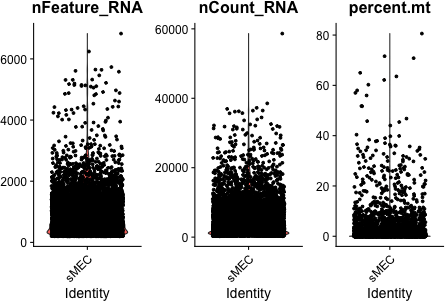
\includegraphics{figures/pre-processing-1.png}
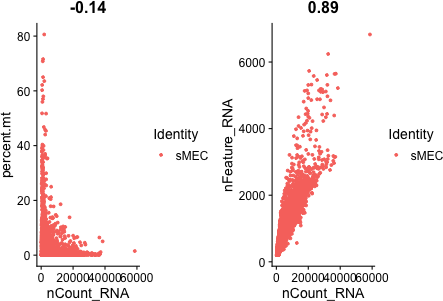
\includegraphics{figures/pre-processing-2.png} \#\# Normalizing Data

Normalizes the feature expression for each cell by the total expression
x 1000, then log transforms

\hypertarget{highly-variable-features}{%
\subsection{Highly Variable Features}\label{highly-variable-features}}

Features with high cell to cell variability (highly expressed in some
cells but not others)

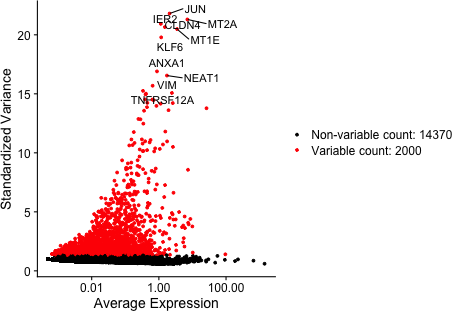
\includegraphics{figures/variable-features-1.png}

\hypertarget{scaling}{%
\subsection{Scaling}\label{scaling}}

Shifts expression so that mean expression across cells is 0, and
variance is 1. This reduces the impact of outliers on downstream
analyses. We did not regress out specific sources of heterogeneity like
mitochondrial contamination or cell cycle stage.

\hypertarget{dimensionality-reductions}{%
\section{Dimensionality Reductions}\label{dimensionality-reductions}}

\begin{verbatim}
## PC_ 1 
## Positive:  SPP1, CLU, SCGB3A1, HPGD, MYBPC1 
## Negative:  MALAT1, NEAT1, KLF6, JUNB, BTG1 
## PC_ 2 
## Positive:  CLDN4, TNFRSF12A, ELF3, MT1E, ATF3 
## Negative:  SRGN, PTPRC, LAPTM5, CD52, CXCR4 
## PC_ 3 
## Positive:  TYROBP, FCER1G, SPI1, CD68, FABP5 
## Negative:  ETS1, TRAC, CD3E, CD2, FYN 
## PC_ 4 
## Positive:  KIAA0101, TYMS, PTTG1, STMN1, CCNB1 
## Negative:  NEAT1, MT-CO3, MT-CO1, MT-ND4, XIST 
## PC_ 5 
## Positive:  S100A10, S100A6, FTL, S100A4, HCST 
## Negative:  KIAA0101, BIRC5, CCNB1, TYMS, TOP2A
\end{verbatim}

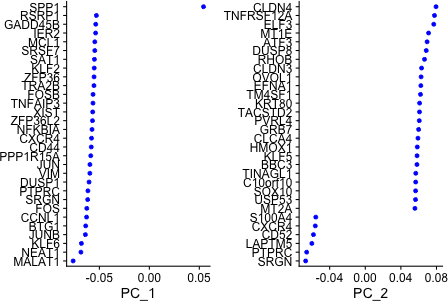
\includegraphics{figures/dimensionality-pca-1.png}
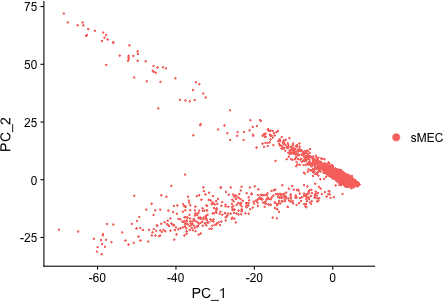
\includegraphics{figures/dimensionality-pca-2.png}
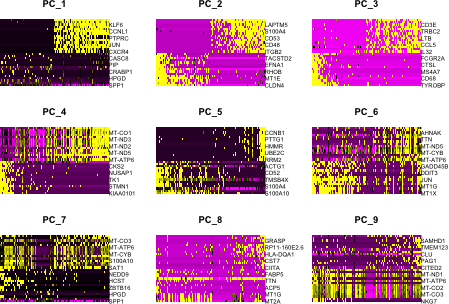
\includegraphics{figures/dimensionality-pca-3.png}

\hypertarget{determination-of-number-of-clusters}{%
\section{Determination of Number of
Clusters}\label{determination-of-number-of-clusters}}

Used the JackStraw procedure in Macosko et al. (2015), sampling 1\% of
the data re-running the PCA and constructing a null distribution of
feature scores, then repeating. This identified `significant' PCs. We
also did an elbow plot.

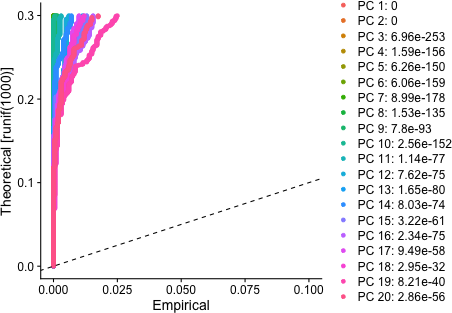
\includegraphics{figures/cluster-numbers-1.png}
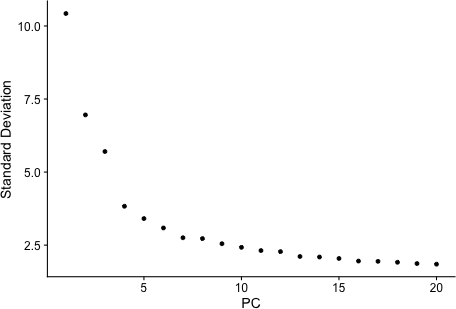
\includegraphics{figures/cluster-numbers-2.png}

Based on this we decided to use 7 PCs to cluster the cells.

\hypertarget{clustering-cell-types}{%
\section{Clustering Cell Types}\label{clustering-cell-types}}

Seurat 3.2 uses a K-nearest neighbor approach then tries to partition
this into commmunities of cell types.

\hypertarget{identification-and-assignment-of-clusters}{%
\subsection{Identification and Assignment of
Clusters}\label{identification-and-assignment-of-clusters}}

\begin{verbatim}
## Modularity Optimizer version 1.3.0 by Ludo Waltman and Nees Jan van Eck
## 
## Number of nodes: 5917
## Number of edges: 178451
## 
## Running Louvain algorithm...
## Maximum modularity in 10 random starts: 0.7940
## Number of communities: 13
## Elapsed time: 0 seconds
\end{verbatim}

\hypertarget{non-linear-dimensionality-reduction}{%
\subsection{Non-Linear Dimensionality
Reduction}\label{non-linear-dimensionality-reduction}}

Did both UMAP and t-SNE plots using 7 clusters

\hypertarget{t-sne-plots}{%
\subsubsection{t-SNE Plots}\label{t-sne-plots}}

\begin{figure}
\centering
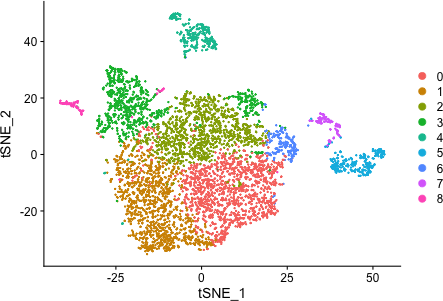
\includegraphics{figures/tsne-plot-initial-1.png}
\caption{t-SNE plot of secreted MECs}
\end{figure}

\hypertarget{umap}{%
\subsubsection{UMAP}\label{umap}}

\begin{figure}
\centering
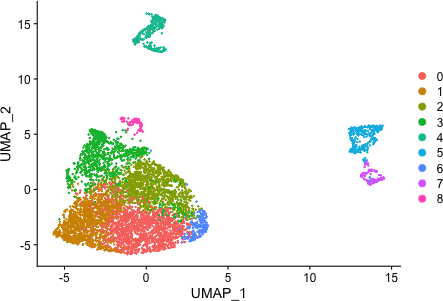
\includegraphics{figures/umap-plot-initial-1.png}
\caption{UMAP plot of secreted MECs}
\end{figure}

\begin{longtable}[]{@{}rrrrrll@{}}
\caption{Cell Specific Markers (All)}\tabularnewline
\toprule
p\_val & avg\_logFC & pct.1 & pct.2 & p\_val\_adj & cluster &
gene\tabularnewline
\midrule
\endfirsthead
\toprule
p\_val & avg\_logFC & pct.1 & pct.2 & p\_val\_adj & cluster &
gene\tabularnewline
\midrule
\endhead
0 & 0.916 & 0.611 & 0.176 & 0 & 4 & LY6D\tabularnewline
0 & 1.109 & 0.892 & 0.592 & 0 & 4 & CLU\tabularnewline
0 & 0.888 & 0.542 & 0.186 & 0 & 4 & KRT15\tabularnewline
0 & 3.261 & 0.997 & 0.137 & 0 & 5 & MALAT1\tabularnewline
0 & 2.638 & 0.772 & 0.012 & 0 & 5 & PTPRC\tabularnewline
0 & 2.774 & 0.994 & 0.545 & 0 & 5 & MT-ATP6\tabularnewline
0 & 2.964 & 0.846 & 0.085 & 0 & 6 & JUN\tabularnewline
0 & 3.724 & 0.643 & 0.050 & 0 & 6 & MT1E\tabularnewline
0 & 3.935 & 0.750 & 0.111 & 0 & 6 & MT2A\tabularnewline
0 & 1.590 & 1.000 & 0.664 & 0 & 7 & MT-CO1\tabularnewline
0 & 1.430 & 1.000 & 0.650 & 0 & 7 & MT-CO3\tabularnewline
0 & 1.373 & 0.860 & 0.358 & 0 & 7 & MT-ND5\tabularnewline
0 & 2.329 & 0.715 & 0.046 & 0 & 8 & DEFB1\tabularnewline
0 & 1.624 & 0.951 & 0.250 & 0 & 8 & KRT7\tabularnewline
0 & 2.003 & 0.812 & 0.215 & 0 & 8 & KRT15\tabularnewline
0 & 3.098 & 0.801 & 0.054 & 0 & 9 & VIM\tabularnewline
0 & 3.122 & 0.823 & 0.422 & 0 & 9 & CD74\tabularnewline
0 & 3.147 & 0.908 & 0.834 & 0 & 9 & FTL\tabularnewline
0 & 1.997 & 0.745 & 0.082 & 0 & 10 & STMN1\tabularnewline
0 & 1.974 & 0.816 & 0.319 & 0 & 10 & H2AFZ\tabularnewline
0 & 1.914 & 0.857 & 0.474 & 0 & 10 & TUBA1B\tabularnewline
0 & 1.301 & 1.000 & 0.805 & 0 & 11 & XDH\tabularnewline
0 & 1.439 & 1.000 & 0.755 & 0 & 11 & FASN\tabularnewline
0 & 1.067 & 0.912 & 0.604 & 0 & 11 & BTN1A1\tabularnewline
0 & 3.137 & 0.882 & 0.070 & 0 & 12 & MT1E\tabularnewline
0 & 3.030 & 0.725 & 0.070 & 0 & 12 & MT1X\tabularnewline
0 & 3.073 & 0.922 & 0.133 & 0 & 12 & MT2A\tabularnewline
\bottomrule
\end{longtable}

\hypertarget{feature-analysis}{%
\section{Feature Analysis}\label{feature-analysis}}

\hypertarget{annotation-of-clusters}{%
\subsection{Annotation of clusters}\label{annotation-of-clusters}}

Used for cell marker enrichment

Used CellMarker for enrichment analyses
\url{http://bio-bigdata.hrbmu.edu.cn/CellMarker/download/Human_cell_markers.txt}.
See Zhang et al. (2019) and
\url{http://bio-bigdata.hrbmu.edu.cn/CellMarker} for details on this
resource

\hypertarget{cluster-5}{%
\subsubsection{Cluster 5}\label{cluster-5}}

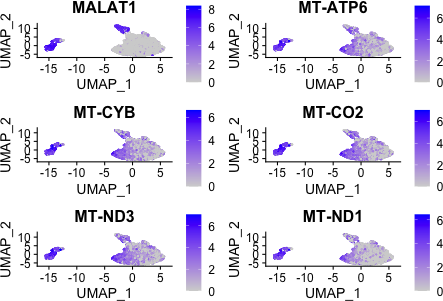
\includegraphics{figures/cluster-annotation-5-1.png}
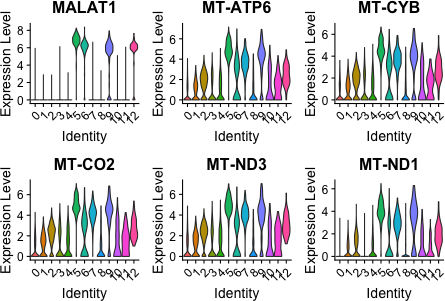
\includegraphics{figures/cluster-annotation-5-2.png}

\begin{longtable}[]{@{}lllrrrrrrrll@{}}
\toprule
\begin{minipage}[b]{0.01\columnwidth}\raggedright
\strut
\end{minipage} & \begin{minipage}[b]{0.01\columnwidth}\raggedright
ID\strut
\end{minipage} & \begin{minipage}[b]{0.01\columnwidth}\raggedright
Description\strut
\end{minipage} & \begin{minipage}[b]{0.00\columnwidth}\raggedleft
setSize\strut
\end{minipage} & \begin{minipage}[b]{0.00\columnwidth}\raggedleft
enrichmentScore\strut
\end{minipage} & \begin{minipage}[b]{0.00\columnwidth}\raggedleft
NES\strut
\end{minipage} & \begin{minipage}[b]{0.00\columnwidth}\raggedleft
pvalue\strut
\end{minipage} & \begin{minipage}[b]{0.00\columnwidth}\raggedleft
p.adjust\strut
\end{minipage} & \begin{minipage}[b]{0.00\columnwidth}\raggedleft
qvalues\strut
\end{minipage} & \begin{minipage}[b]{0.00\columnwidth}\raggedleft
rank\strut
\end{minipage} & \begin{minipage}[b]{0.01\columnwidth}\raggedright
leading\_edge\strut
\end{minipage} & \begin{minipage}[b]{0.63\columnwidth}\raggedright
core\_enrichment\strut
\end{minipage}\tabularnewline
\midrule
\endhead
\begin{minipage}[t]{0.01\columnwidth}\raggedright
Fetal kidney, Normal, Natural killer T (NKT) cell\strut
\end{minipage} & \begin{minipage}[t]{0.01\columnwidth}\raggedright
Fetal kidney, Normal, Natural killer T (NKT) cell\strut
\end{minipage} & \begin{minipage}[t]{0.01\columnwidth}\raggedright
Fetal kidney, Normal, Natural killer T (NKT) cell\strut
\end{minipage} & \begin{minipage}[t]{0.00\columnwidth}\raggedleft
399\strut
\end{minipage} & \begin{minipage}[t]{0.00\columnwidth}\raggedleft
-0.222\strut
\end{minipage} & \begin{minipage}[t]{0.00\columnwidth}\raggedleft
-2.19\strut
\end{minipage} & \begin{minipage}[t]{0.00\columnwidth}\raggedleft
0.001\strut
\end{minipage} & \begin{minipage}[t]{0.00\columnwidth}\raggedleft
0.016\strut
\end{minipage} & \begin{minipage}[t]{0.00\columnwidth}\raggedleft
0.015\strut
\end{minipage} & \begin{minipage}[t]{0.00\columnwidth}\raggedleft
436\strut
\end{minipage} & \begin{minipage}[t]{0.01\columnwidth}\raggedright
tags=99\%, list=96\%, signal=30\%\strut
\end{minipage} & \begin{minipage}[t]{0.63\columnwidth}\raggedright
TTN/SYNE2/HLA-B/IL32/CXCR4/ZFP36L2/RNF213/SRGN/HLA-A/STK4/LTB/CD44/TNFAIP3/NKTR/ETS1/IL7R/EML4/HLA-E/PRRC2C/CD52/FYN/S100A4/IRF1/B2M/ANKRD11/PIK3R1/ANKRD12/CCNL1/SRSF7/CD2/JUNB/MBNL1/TRA2B/DDX5/CD69/RBM39/RORA/SLC2A3/ARID4B/CLEC2D/ARHGDIB/ID2/KMT2E/NFKBIA/ARL4C/STK17B/CREM/REL/CYLD/CNOT6L/HLA-C/FUS/SRSF11/CORO1A/MACF1/AHNAK/EVL/ATRX/TXNIP/USP15/TNRC6B/PPP2R5C/CD3E/SRSF5/KLF6/BPTF/CYTIP/SPOCK2/PNISR/RUNX3/CELF2/TSC22D3/JAK1/RSRP1/SMG1/AKAP13/GOLGA8B/DDX3X/FAM133B/SAMSN1/HNRNPH1/AKAP9/CD3D/NR4A2/PRPF38B/FOXP1/GCC2/UTRN/CD247/FOS/ITK/SRRM2/RGS1/CLK1/ARGLU1/RPS27/XAF1/CDC42SE2/CYBA/PTMA/CD7/ZC3HAV1/SLC38A1/RBM25/WIPF1/RASGRP1/PDE4B/PPP1R15A/VIM/AKNA/FNBP1/IL2RG/TSPYL2/PCSK7/ARID5B/DDX24/GOLGB1/HCST/FLNA/ITGB1/CYTH1/SLC38A2/KIAA1551/CHD1/TGFB1/DUSP2/KIAA1109/JUN/CD48/AAK1/GBP5/SF3B1/SON/PBXIP1/FAM129A/RNF19A/HMGB2/IDS/SYTL3/ARAP2/TPR/ITGA4/BCL11B/SLFN5/MPHOSPH8/TLE4/ACAP1/MBP/LUC7L3/LAPTM5/PRPF4B/ATM/RHOH/DDX17/ZNF292/BRD2/LEPROTL1/SARAF/RNF149/ISG15/CD99/HIST1H4C/N4BP2L2/BCLAF1/FXYD5/ATP2B1/LIMD2/PARP8/TNFRSF1B/PCM1/LSP1/SF1/GOLGA4/GNG2/WSB1/LYST/DHX36/KMT2A/ASH1L/BDP1/CHD2/FNBP4/ITSN2/JUND/SRRM1/EIF3A/POLR2J3/HLA-F/RNF125/SP100/LCK/CD53/FMNL1/NCL/KMT2C/DUSP1/RNMT/PIM1/SMAP2/ADGRE5/BTG2/HNRNPDL/BOD1L1/SFPQ/GMFG/ELF1/VPS13C/SCAF11/RSRC2/ZFP36L1/SRSF3/GIMAP7/NIPBL/PLCG2/RBBP6/EMB/BAZ1A/STK17A/NOP58/IKZF1/CFLAR/KDM2A/MECP2/RPS19/PRKX/RAC2/YTHDC1/PRDM2/CD37/MYCBP2/RBM5/AES/USP34/PTPN22/RBM6/JMJD1C/ZNF207/DNAJB1/RB1CC1/TAF1D/ANKRD44/YWHAB/SAFB2/G3BP2/SPTAN1/CLEC2B/COTL1/PNN/S100A10/MCL1/NCOR1/PHF3/GADD45B/IFITM1/SRSF10/ARHGEF1/ZC3H13/EIF5B/PTGER4/ADAR/EPC1/DDX6/ZFP36/LITAF/DDX46/PPP1R12A/PPP1R10/WNK1/GLS/MTRNR2L8/LRRFIP1/TRA2A/TMF1/YWHAZ/PRKCH/NFE2L2/YPEL5/ARHGAP15/RSF1/NAP1L4/GPBP1/NOP56/EMP3/H3F3B/HP1BP3/NSMCE3/APBB1IP/LCP1/TPM3/HNRNPU/MYH9/OFD1/ODF2L/SRSF2/KTN1/CREBRF/HMGB1/ITGB2/EIF5/YME1L1/FAU/NAP1L1/RTF1/PARP14/IFITM2/TCF25/BRD4/ROCK1/DDX21/THRAP3/RAD21/CALM1/IER5/PTPN2/GPSM3/SLTM/PAK2/NASP/DNAJA1/FOXN3/OPTN/HNRNPUL1/ANP32B/CDKN1B/IVNS1ABP/MTDH/IFRD1/PRPF40A/ARPC2/SH3BGRL3/HNRNPC/PNRC1/RAP1B/RPS29/RPS3/HNRNPA2B1/PTP4A2/PIK3IP1/CDC42SE1/TTC39C/VAMP2/ICAM3/EIF4G2/PPIG/TUBA4A/TERF2IP/ORMDL1/ISG20/BRD7/C9orf78/GSPT1/HERPUD1/GGNBP2/PFN1/IK/RBMX/C6orf48/RHOG/RPL28/SYAP1/PCBP2/ARF6/IER2/EZR/SF3B2/DDX18/RPS21/GNAI2/LDHA/EIF1/RPSA/NR3C1/SYF2/TAPBP/ACTR2/RPS27A/RPS15A/SNRNP70/KIF5B/ABHD17A/MAP1LC3B/UBALD2/METAP2/SUB1/DEK/HNRNPA3/TUBB4B/DPP7/H1FX/EIF4A2/SET/IQGAP1/PLP2/UBXN4/TTC3\strut
\end{minipage}\tabularnewline
\bottomrule
\end{longtable}

\hypertarget{cluster-9}{%
\subsubsection{Cluster 9}\label{cluster-9}}

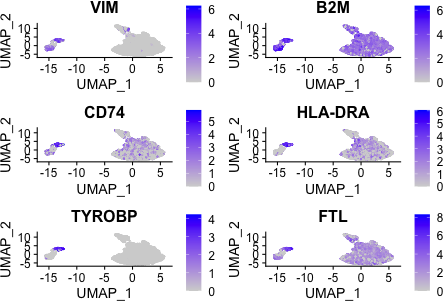
\includegraphics{figures/cluster-annotation-9-1.png}
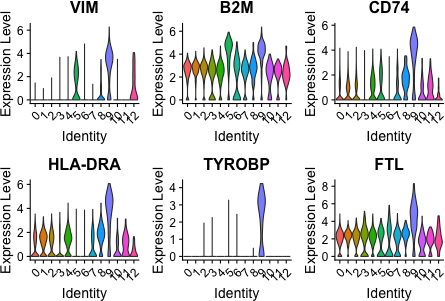
\includegraphics{figures/cluster-annotation-9-2.png}

\begin{longtable}[]{@{}lllrrrrrrrll@{}}
\toprule
\begin{minipage}[b]{0.03\columnwidth}\raggedright
\strut
\end{minipage} & \begin{minipage}[b]{0.03\columnwidth}\raggedright
ID\strut
\end{minipage} & \begin{minipage}[b]{0.03\columnwidth}\raggedright
Description\strut
\end{minipage} & \begin{minipage}[b]{0.00\columnwidth}\raggedleft
setSize\strut
\end{minipage} & \begin{minipage}[b]{0.01\columnwidth}\raggedleft
enrichmentScore\strut
\end{minipage} & \begin{minipage}[b]{0.00\columnwidth}\raggedleft
NES\strut
\end{minipage} & \begin{minipage}[b]{0.00\columnwidth}\raggedleft
pvalue\strut
\end{minipage} & \begin{minipage}[b]{0.01\columnwidth}\raggedleft
p.adjust\strut
\end{minipage} & \begin{minipage}[b]{0.00\columnwidth}\raggedleft
qvalues\strut
\end{minipage} & \begin{minipage}[b]{0.00\columnwidth}\raggedleft
rank\strut
\end{minipage} & \begin{minipage}[b]{0.02\columnwidth}\raggedright
leading\_edge\strut
\end{minipage} & \begin{minipage}[b]{0.55\columnwidth}\raggedright
core\_enrichment\strut
\end{minipage}\tabularnewline
\midrule
\endhead
\begin{minipage}[t]{0.03\columnwidth}\raggedright
Lung, Normal, Secretory cell\strut
\end{minipage} & \begin{minipage}[t]{0.03\columnwidth}\raggedright
Lung, Normal, Secretory cell\strut
\end{minipage} & \begin{minipage}[t]{0.03\columnwidth}\raggedright
Lung, Normal, Secretory cell\strut
\end{minipage} & \begin{minipage}[t]{0.00\columnwidth}\raggedleft
15\strut
\end{minipage} & \begin{minipage}[t]{0.01\columnwidth}\raggedleft
0.717\strut
\end{minipage} & \begin{minipage}[t]{0.00\columnwidth}\raggedleft
2.27\strut
\end{minipage} & \begin{minipage}[t]{0.00\columnwidth}\raggedleft
0.000\strut
\end{minipage} & \begin{minipage}[t]{0.01\columnwidth}\raggedleft
0.000\strut
\end{minipage} & \begin{minipage}[t]{0.00\columnwidth}\raggedleft
0.000\strut
\end{minipage} & \begin{minipage}[t]{0.00\columnwidth}\raggedleft
60\strut
\end{minipage} & \begin{minipage}[t]{0.02\columnwidth}\raggedright
tags=67\%, list=14\%, signal=59\%\strut
\end{minipage} & \begin{minipage}[t]{0.55\columnwidth}\raggedright
CD74/HLA-DPA1/HLA-DQA1/HLA-DRA/HLA-DRB1/HLA-DPB1/HLA-DQB1/HLA-DRB5/CXCL8/HLA-A\strut
\end{minipage}\tabularnewline
\begin{minipage}[t]{0.03\columnwidth}\raggedright
Embryonic prefrontal cortex, Normal, Microglial cell\strut
\end{minipage} & \begin{minipage}[t]{0.03\columnwidth}\raggedright
Embryonic prefrontal cortex, Normal, Microglial cell\strut
\end{minipage} & \begin{minipage}[t]{0.03\columnwidth}\raggedright
Embryonic prefrontal cortex, Normal, Microglial cell\strut
\end{minipage} & \begin{minipage}[t]{0.00\columnwidth}\raggedleft
124\strut
\end{minipage} & \begin{minipage}[t]{0.01\columnwidth}\raggedleft
0.413\strut
\end{minipage} & \begin{minipage}[t]{0.00\columnwidth}\raggedleft
1.81\strut
\end{minipage} & \begin{minipage}[t]{0.00\columnwidth}\raggedleft
0.000\strut
\end{minipage} & \begin{minipage}[t]{0.01\columnwidth}\raggedleft
0.001\strut
\end{minipage} & \begin{minipage}[t]{0.00\columnwidth}\raggedleft
0.000\strut
\end{minipage} & \begin{minipage}[t]{0.00\columnwidth}\raggedleft
182\strut
\end{minipage} & \begin{minipage}[t]{0.02\columnwidth}\raggedright
tags=60\%, list=43\%, signal=49\%\strut
\end{minipage} & \begin{minipage}[t]{0.55\columnwidth}\raggedright
FTL/CD74/TYROBP/FABP5/CTSD/FCER1G/SRGN/SAT1/CTSB/APOC1/CTSL/CD68/NFKBIA/LAPTM5/FOS/CD83/HLA-B/GPX1/CYBA/AIF1/NPC2/RGS1/CCL3/GPR183/CTSS/ITGB2/FOSB/GADD45B/HCST/B2M/ASAH1/PLEK/SGK1/RGS2/FCGRT/IER3/RNF130/DUSP1/GRN/S100A11/CPVL/ZFP36/LCP1/PFN1/CXCL16/ITGAX/MGAT1/GMFG/ANXA5/CEBPD/CD53/HLA-C/IGSF6/MS4A7/ARRB2/LST1/APLP2/UCP2/CD86/RGS10/BRI3/JUNB/ARHGDIB/GNAI2/CD37/HEXB/PLA2G7/PTPRC/KLF6/CTSA/LIMS1/FCGR2A/HAVCR2/PSAP/HLA-E\strut
\end{minipage}\tabularnewline
\begin{minipage}[t]{0.03\columnwidth}\raggedright
Large intestine, Normal, Paneth cell\strut
\end{minipage} & \begin{minipage}[t]{0.03\columnwidth}\raggedright
Large intestine, Normal, Paneth cell\strut
\end{minipage} & \begin{minipage}[t]{0.03\columnwidth}\raggedright
Large intestine, Normal, Paneth cell\strut
\end{minipage} & \begin{minipage}[t]{0.00\columnwidth}\raggedleft
81\strut
\end{minipage} & \begin{minipage}[t]{0.01\columnwidth}\raggedleft
0.462\strut
\end{minipage} & \begin{minipage}[t]{0.00\columnwidth}\raggedleft
1.97\strut
\end{minipage} & \begin{minipage}[t]{0.00\columnwidth}\raggedleft
0.000\strut
\end{minipage} & \begin{minipage}[t]{0.01\columnwidth}\raggedleft
0.001\strut
\end{minipage} & \begin{minipage}[t]{0.00\columnwidth}\raggedleft
0.000\strut
\end{minipage} & \begin{minipage}[t]{0.00\columnwidth}\raggedleft
144\strut
\end{minipage} & \begin{minipage}[t]{0.02\columnwidth}\raggedright
tags=58\%, list=34\%, signal=47\%\strut
\end{minipage} & \begin{minipage}[t]{0.55\columnwidth}\raggedright
CD74/HLA-DPA1/HLA-DQA1/HLA-DRA/HLA-DRB1/TYROBP/HLA-DPB1/FCER1G/SRGN/HLA-DQB1/CTSL/CD68/LAPTM5/SOD2/CD83/AIF1/CTSZ/CXCL8/CCL3/ITGB2/PLAUR/HCST/PLEK/COTL1/SGK1/ACP5/SPI1/BCL2A1/CPVL/HLA-DMB/CD48/LCP1/LSP1/CEBPB/CXCL16/ITGAX/METRNL/GMFG/CD53/SLAMF7/IGSF6/MS4A7/ARRB2/LST1/UCP2/CD86/LYZ\strut
\end{minipage}\tabularnewline
\begin{minipage}[t]{0.03\columnwidth}\raggedright
Fetal kidney, Normal, Monocyte\strut
\end{minipage} & \begin{minipage}[t]{0.03\columnwidth}\raggedright
Fetal kidney, Normal, Monocyte\strut
\end{minipage} & \begin{minipage}[t]{0.03\columnwidth}\raggedright
Fetal kidney, Normal, Monocyte\strut
\end{minipage} & \begin{minipage}[t]{0.00\columnwidth}\raggedleft
212\strut
\end{minipage} & \begin{minipage}[t]{0.01\columnwidth}\raggedleft
0.367\strut
\end{minipage} & \begin{minipage}[t]{0.00\columnwidth}\raggedleft
1.64\strut
\end{minipage} & \begin{minipage}[t]{0.00\columnwidth}\raggedleft
0.001\strut
\end{minipage} & \begin{minipage}[t]{0.01\columnwidth}\raggedleft
0.005\strut
\end{minipage} & \begin{minipage}[t]{0.00\columnwidth}\raggedleft
0.004\strut
\end{minipage} & \begin{minipage}[t]{0.00\columnwidth}\raggedleft
269\strut
\end{minipage} & \begin{minipage}[t]{0.02\columnwidth}\raggedright
tags=76\%, list=63\%, signal=56\%\strut
\end{minipage} & \begin{minipage}[t]{0.55\columnwidth}\raggedright
CD74/VIM/HLA-DRA/HLA-DRB1/TYROBP/CTSD/LGALS1/FCER1G/SRGN/SAT1/TIMP1/CTSB/C15orf48/CD68/NFKBIA/S100A4/LAPTM5/HLA-DRB5/SOD2/CD83/TYMP/HLA-B/GPX1/CYBA/AIF1/CXCL8/EMP3/CTSS/LGALS3/BTG1/HLA-A/ITGB2/BASP1/S100A10/CD52/FOSB/PLAUR/CAPG/S100A6/HCST/ASAH1/SH3BGRL3/PLEK/COTL1/GSTO1/ZEB2/RGS2/FCGRT/IER3/RNF130/DUSP1/SPI1/GRN/BCL2A1/S100A11/CPVL/ZFP36/CD48/CD44/LCP1/TGFBI/HIF1A/LSP1/SERPINB1/CEBPB/CXCL16/ITGAX/GMFG/ANXA5/CEBPD/CD53/CCNL1/PHACTR1/LITAF/HLA-C/IGSF6/MS4A7/ARRB2/LST1/CST3/PKM/CTSH/APLP2/CD86/RGS10/BRI3/LYZ/PPP1R15A/PLSCR1/ANXA1/ANXA2/KLF4/FXYD5/LRRFIP1/SAMHD1/ARHGDIB/GNAI2/CD37/MS4A6A/BID/EFHD2/C1orf162/PTPRC/ATP6V0B/KLF6/OAZ1/LIMS1/FCGR2A/PSAP/TPM3/HLA-E/IFI30/JAML/RAB31/CFLAR/FMNL1/NAMPT/SLC16A3/EMILIN2/GLUL/ALDH2/NINJ1/ATP2B1/WARS/PTP4A2/SAMSN1/PTPRE/SRSF5/GLIPR1/SDCBP/MCL1/LYN/C4orf48/GRINA/IFNGR1/GRB2/ZFAND5/CAP1/DNAJA1/ARPC2/HLA-DMA/CD63/RNASET2/QKI/VMP1/PFDN5/MTRNR2L8/RILPL2/RNH1/TXN/GPSM3/TNFAIP3/G0S2/ATP6V1B2/GK/FAM49B/KYNU/CLEC7A/CNPY3/UBA52/MARCKS/IFITM2\strut
\end{minipage}\tabularnewline
\begin{minipage}[t]{0.03\columnwidth}\raggedright
Kidney, Renal Cell Carcinoma, B cell\strut
\end{minipage} & \begin{minipage}[t]{0.03\columnwidth}\raggedright
Kidney, Renal Cell Carcinoma, B cell\strut
\end{minipage} & \begin{minipage}[t]{0.03\columnwidth}\raggedright
Kidney, Renal Cell Carcinoma, B cell\strut
\end{minipage} & \begin{minipage}[t]{0.00\columnwidth}\raggedleft
23\strut
\end{minipage} & \begin{minipage}[t]{0.01\columnwidth}\raggedleft
0.577\strut
\end{minipage} & \begin{minipage}[t]{0.00\columnwidth}\raggedleft
2.04\strut
\end{minipage} & \begin{minipage}[t]{0.00\columnwidth}\raggedleft
0.001\strut
\end{minipage} & \begin{minipage}[t]{0.01\columnwidth}\raggedleft
0.005\strut
\end{minipage} & \begin{minipage}[t]{0.00\columnwidth}\raggedleft
0.004\strut
\end{minipage} & \begin{minipage}[t]{0.00\columnwidth}\raggedleft
65\strut
\end{minipage} & \begin{minipage}[t]{0.02\columnwidth}\raggedright
tags=48\%, list=15\%, signal=43\%\strut
\end{minipage} & \begin{minipage}[t]{0.55\columnwidth}\raggedright
CD74/HLA-DPA1/HLA-DQA1/HLA-DRA/HLA-DRB1/HLA-DPB1/HLA-DQB1/HLA-DRB5/CD83/GPR183/CD52\strut
\end{minipage}\tabularnewline
\begin{minipage}[t]{0.03\columnwidth}\raggedright
Kidney, Normal, B cell\strut
\end{minipage} & \begin{minipage}[t]{0.03\columnwidth}\raggedright
Kidney, Normal, B cell\strut
\end{minipage} & \begin{minipage}[t]{0.03\columnwidth}\raggedright
Kidney, Normal, B cell\strut
\end{minipage} & \begin{minipage}[t]{0.00\columnwidth}\raggedleft
38\strut
\end{minipage} & \begin{minipage}[t]{0.01\columnwidth}\raggedleft
0.477\strut
\end{minipage} & \begin{minipage}[t]{0.00\columnwidth}\raggedleft
1.84\strut
\end{minipage} & \begin{minipage}[t]{0.00\columnwidth}\raggedleft
0.001\strut
\end{minipage} & \begin{minipage}[t]{0.01\columnwidth}\raggedleft
0.008\strut
\end{minipage} & \begin{minipage}[t]{0.00\columnwidth}\raggedleft
0.006\strut
\end{minipage} & \begin{minipage}[t]{0.00\columnwidth}\raggedleft
69\strut
\end{minipage} & \begin{minipage}[t]{0.02\columnwidth}\raggedright
tags=37\%, list=16\%, signal=34\%\strut
\end{minipage} & \begin{minipage}[t]{0.55\columnwidth}\raggedright
CD74/HLA-DPA1/HLA-DQA1/HLA-DRA/HLA-DRB1/HLA-DPB1/HLA-DQB1/LAPTM5/HLA-DRB5/CD83/GPR183/BASP1/CD52/CAPG\strut
\end{minipage}\tabularnewline
\begin{minipage}[t]{0.03\columnwidth}\raggedright
Kidney, Renal Cell Carcinoma, Neutrophil\strut
\end{minipage} & \begin{minipage}[t]{0.03\columnwidth}\raggedright
Kidney, Renal Cell Carcinoma, Neutrophil\strut
\end{minipage} & \begin{minipage}[t]{0.03\columnwidth}\raggedright
Kidney, Renal Cell Carcinoma, Neutrophil\strut
\end{minipage} & \begin{minipage}[t]{0.00\columnwidth}\raggedleft
17\strut
\end{minipage} & \begin{minipage}[t]{0.01\columnwidth}\raggedleft
0.550\strut
\end{minipage} & \begin{minipage}[t]{0.00\columnwidth}\raggedleft
1.80\strut
\end{minipage} & \begin{minipage}[t]{0.00\columnwidth}\raggedleft
0.008\strut
\end{minipage} & \begin{minipage}[t]{0.01\columnwidth}\raggedleft
0.045\strut
\end{minipage} & \begin{minipage}[t]{0.00\columnwidth}\raggedleft
0.035\strut
\end{minipage} & \begin{minipage}[t]{0.00\columnwidth}\raggedleft
134\strut
\end{minipage} & \begin{minipage}[t]{0.02\columnwidth}\raggedright
tags=71\%, list=31\%, signal=50\%\strut
\end{minipage} & \begin{minipage}[t]{0.55\columnwidth}\raggedright
FTL/TYROBP/SAT1/SOD2/FOS/CXCL8/RGS2/BCL2A1/S100A11/CEBPB/IGSF6/LST1\strut
\end{minipage}\tabularnewline
\bottomrule
\end{longtable}

\hypertarget{cluster-6}{%
\subsubsection{Cluster 6}\label{cluster-6}}

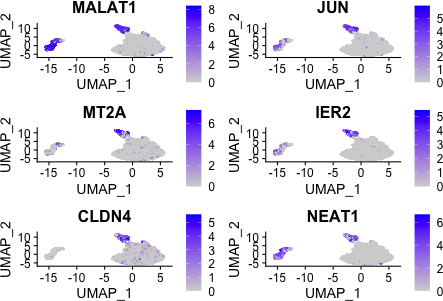
\includegraphics{figures/cluster-annotation-6-1.png}
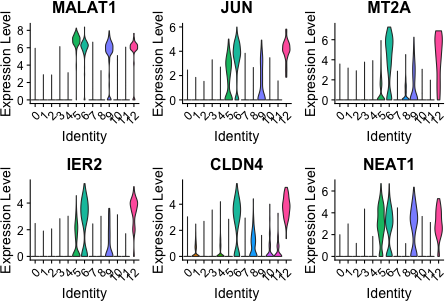
\includegraphics{figures/cluster-annotation-6-2.png}

\begin{longtable}[]{@{}lllrrrrrrrll@{}}
\toprule
\begin{minipage}[b]{0.11\columnwidth}\raggedright
\strut
\end{minipage} & \begin{minipage}[b]{0.11\columnwidth}\raggedright
ID\strut
\end{minipage} & \begin{minipage}[b]{0.11\columnwidth}\raggedright
Description\strut
\end{minipage} & \begin{minipage}[b]{0.02\columnwidth}\raggedleft
setSize\strut
\end{minipage} & \begin{minipage}[b]{0.03\columnwidth}\raggedleft
enrichmentScore\strut
\end{minipage} & \begin{minipage}[b]{0.01\columnwidth}\raggedleft
NES\strut
\end{minipage} & \begin{minipage}[b]{0.01\columnwidth}\raggedleft
pvalue\strut
\end{minipage} & \begin{minipage}[b]{0.02\columnwidth}\raggedleft
p.adjust\strut
\end{minipage} & \begin{minipage}[b]{0.02\columnwidth}\raggedleft
qvalues\strut
\end{minipage} & \begin{minipage}[b]{0.01\columnwidth}\raggedleft
rank\strut
\end{minipage} & \begin{minipage}[b]{0.06\columnwidth}\raggedright
leading\_edge\strut
\end{minipage} & \begin{minipage}[b]{0.20\columnwidth}\raggedright
core\_enrichment\strut
\end{minipage}\tabularnewline
\midrule
\endhead
\begin{minipage}[t]{0.11\columnwidth}\raggedright
Brain, Normal, Astrocyte\strut
\end{minipage} & \begin{minipage}[t]{0.11\columnwidth}\raggedright
Brain, Normal, Astrocyte\strut
\end{minipage} & \begin{minipage}[t]{0.11\columnwidth}\raggedright
Brain, Normal, Astrocyte\strut
\end{minipage} & \begin{minipage}[t]{0.02\columnwidth}\raggedleft
16\strut
\end{minipage} & \begin{minipage}[t]{0.03\columnwidth}\raggedleft
0.722\strut
\end{minipage} & \begin{minipage}[t]{0.01\columnwidth}\raggedleft
2.13\strut
\end{minipage} & \begin{minipage}[t]{0.01\columnwidth}\raggedleft
0\strut
\end{minipage} & \begin{minipage}[t]{0.02\columnwidth}\raggedleft
0.000\strut
\end{minipage} & \begin{minipage}[t]{0.02\columnwidth}\raggedleft
0.000\strut
\end{minipage} & \begin{minipage}[t]{0.01\columnwidth}\raggedleft
46\strut
\end{minipage} & \begin{minipage}[t]{0.06\columnwidth}\raggedright
tags=94\%, list=32\%, signal=71\%\strut
\end{minipage} & \begin{minipage}[t]{0.20\columnwidth}\raggedright
MT2A/MT1X/JUN/IER2/ATF3/JUND/FOS/ZFP36/RHOB/FOSB/JUNB/GADD45B/ZFP36L1/ZFP36L2/NFKBIA\strut
\end{minipage}\tabularnewline
\begin{minipage}[t]{0.11\columnwidth}\raggedright
Embryonic prefrontal cortex, Normal, Microglial cell\strut
\end{minipage} & \begin{minipage}[t]{0.11\columnwidth}\raggedright
Embryonic prefrontal cortex, Normal, Microglial cell\strut
\end{minipage} & \begin{minipage}[t]{0.11\columnwidth}\raggedright
Embryonic prefrontal cortex, Normal, Microglial cell\strut
\end{minipage} & \begin{minipage}[t]{0.02\columnwidth}\raggedleft
20\strut
\end{minipage} & \begin{minipage}[t]{0.03\columnwidth}\raggedleft
0.637\strut
\end{minipage} & \begin{minipage}[t]{0.01\columnwidth}\raggedleft
1.95\strut
\end{minipage} & \begin{minipage}[t]{0.01\columnwidth}\raggedleft
0\strut
\end{minipage} & \begin{minipage}[t]{0.02\columnwidth}\raggedleft
0.001\strut
\end{minipage} & \begin{minipage}[t]{0.02\columnwidth}\raggedleft
0.001\strut
\end{minipage} & \begin{minipage}[t]{0.01\columnwidth}\raggedleft
46\strut
\end{minipage} & \begin{minipage}[t]{0.06\columnwidth}\raggedright
tags=80\%, list=32\%, signal=63\%\strut
\end{minipage} & \begin{minipage}[t]{0.20\columnwidth}\raggedright
JUN/IER2/KLF6/DUSP1/IER3/FOS/ZFP36/RHOB/HIST1H1C/FOSB/S100A11/JUNB/GADD45B/ZFP36L1/ZFP36L2/NFKBIA\strut
\end{minipage}\tabularnewline
\bottomrule
\end{longtable}

\hypertarget{cluster-12}{%
\subsubsection{Cluster 12}\label{cluster-12}}

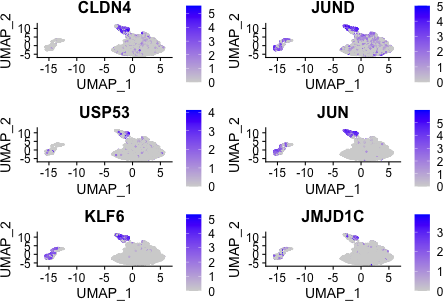
\includegraphics{figures/cluster-annotation-12-1.png}
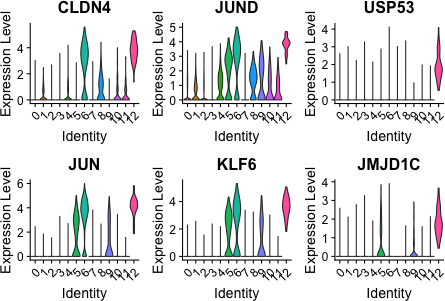
\includegraphics{figures/cluster-annotation-12-2.png}

\begin{longtable}[]{@{}lllrrrrrrrll@{}}
\toprule
\begin{minipage}[b]{0.06\columnwidth}\raggedright
\strut
\end{minipage} & \begin{minipage}[b]{0.06\columnwidth}\raggedright
ID\strut
\end{minipage} & \begin{minipage}[b]{0.06\columnwidth}\raggedright
Description\strut
\end{minipage} & \begin{minipage}[b]{0.01\columnwidth}\raggedleft
setSize\strut
\end{minipage} & \begin{minipage}[b]{0.02\columnwidth}\raggedleft
enrichmentScore\strut
\end{minipage} & \begin{minipage}[b]{0.01\columnwidth}\raggedleft
NES\strut
\end{minipage} & \begin{minipage}[b]{0.01\columnwidth}\raggedleft
pvalue\strut
\end{minipage} & \begin{minipage}[b]{0.01\columnwidth}\raggedleft
p.adjust\strut
\end{minipage} & \begin{minipage}[b]{0.01\columnwidth}\raggedleft
qvalues\strut
\end{minipage} & \begin{minipage}[b]{0.01\columnwidth}\raggedleft
rank\strut
\end{minipage} & \begin{minipage}[b]{0.03\columnwidth}\raggedright
leading\_edge\strut
\end{minipage} & \begin{minipage}[b]{0.40\columnwidth}\raggedright
core\_enrichment\strut
\end{minipage}\tabularnewline
\midrule
\endhead
\begin{minipage}[t]{0.06\columnwidth}\raggedright
Brain, Normal, Astrocyte\strut
\end{minipage} & \begin{minipage}[t]{0.06\columnwidth}\raggedright
Brain, Normal, Astrocyte\strut
\end{minipage} & \begin{minipage}[t]{0.06\columnwidth}\raggedright
Brain, Normal, Astrocyte\strut
\end{minipage} & \begin{minipage}[t]{0.01\columnwidth}\raggedleft
29\strut
\end{minipage} & \begin{minipage}[t]{0.02\columnwidth}\raggedleft
0.723\strut
\end{minipage} & \begin{minipage}[t]{0.01\columnwidth}\raggedleft
2.85\strut
\end{minipage} & \begin{minipage}[t]{0.01\columnwidth}\raggedleft
0.000\strut
\end{minipage} & \begin{minipage}[t]{0.01\columnwidth}\raggedleft
0.000\strut
\end{minipage} & \begin{minipage}[t]{0.01\columnwidth}\raggedleft
0.000\strut
\end{minipage} & \begin{minipage}[t]{0.01\columnwidth}\raggedleft
91\strut
\end{minipage} & \begin{minipage}[t]{0.03\columnwidth}\raggedright
tags=59\%, list=9\%, signal=55\%\strut
\end{minipage} & \begin{minipage}[t]{0.40\columnwidth}\raggedright
MT2A/MT1X/JUN/IER2/RHOB/JUND/FOS/ATF3/ZFP36/JUNB/FOSB/GADD45B/NFKBIA/ZFP36L1/MAFB/ZFP36L2/ZFAND5\strut
\end{minipage}\tabularnewline
\begin{minipage}[t]{0.06\columnwidth}\raggedright
Embryonic prefrontal cortex, Normal, Microglial cell\strut
\end{minipage} & \begin{minipage}[t]{0.06\columnwidth}\raggedright
Embryonic prefrontal cortex, Normal, Microglial cell\strut
\end{minipage} & \begin{minipage}[t]{0.06\columnwidth}\raggedright
Embryonic prefrontal cortex, Normal, Microglial cell\strut
\end{minipage} & \begin{minipage}[t]{0.01\columnwidth}\raggedleft
57\strut
\end{minipage} & \begin{minipage}[t]{0.02\columnwidth}\raggedleft
0.522\strut
\end{minipage} & \begin{minipage}[t]{0.01\columnwidth}\raggedleft
2.34\strut
\end{minipage} & \begin{minipage}[t]{0.01\columnwidth}\raggedleft
0.000\strut
\end{minipage} & \begin{minipage}[t]{0.01\columnwidth}\raggedleft
0.000\strut
\end{minipage} & \begin{minipage}[t]{0.01\columnwidth}\raggedleft
0.000\strut
\end{minipage} & \begin{minipage}[t]{0.01\columnwidth}\raggedleft
151\strut
\end{minipage} & \begin{minipage}[t]{0.03\columnwidth}\raggedright
tags=44\%, list=15\%, signal=40\%\strut
\end{minipage} & \begin{minipage}[t]{0.40\columnwidth}\raggedright
JUN/IER2/KLF6/RHOB/DUSP1/FOS/ZFP36/JUNB/EGR1/FOSB/GADD45B/SOX4/TSC22D1/NFKBIA/HIST1H1C/IER3/S100A11/ZFP36L1/GSN/ZFP36L2/SAT1/SGK1/CEBPD/TUBA1A/NFIB\strut
\end{minipage}\tabularnewline
\begin{minipage}[t]{0.06\columnwidth}\raggedright
Fetal kidney, Normal, Monocyte\strut
\end{minipage} & \begin{minipage}[t]{0.06\columnwidth}\raggedright
Fetal kidney, Normal, Monocyte\strut
\end{minipage} & \begin{minipage}[t]{0.06\columnwidth}\raggedright
Fetal kidney, Normal, Monocyte\strut
\end{minipage} & \begin{minipage}[t]{0.01\columnwidth}\raggedleft
129\strut
\end{minipage} & \begin{minipage}[t]{0.02\columnwidth}\raggedleft
0.407\strut
\end{minipage} & \begin{minipage}[t]{0.01\columnwidth}\raggedleft
1.99\strut
\end{minipage} & \begin{minipage}[t]{0.01\columnwidth}\raggedleft
0.000\strut
\end{minipage} & \begin{minipage}[t]{0.01\columnwidth}\raggedleft
0.000\strut
\end{minipage} & \begin{minipage}[t]{0.01\columnwidth}\raggedleft
0.000\strut
\end{minipage} & \begin{minipage}[t]{0.01\columnwidth}\raggedleft
274\strut
\end{minipage} & \begin{minipage}[t]{0.03\columnwidth}\raggedright
tags=47\%, list=27\%, signal=39\%\strut
\end{minipage} & \begin{minipage}[t]{0.40\columnwidth}\raggedright
IER2/KLF6/ANXA1/JUND/DUSP1/TNFRSF12A/ZFP36/MCL1/PNRC1/PIM3/CEBPB/CITED2/JMJD1C/FOSB/MIDN/ANXA2/SLC3A2/PHLDA2/NFKBIA/S100A6/IER3/S100A11/MAFB/WSB1/S100A10/ZFAND5/FOXO3/PPP1R15A/SRSF3/MAP1LC3B/SAT1/CEBPD/TAGLN2/CCNL1/SLC25A37/PPIF/NAMPT/VIM/LGALS3/TRIB1/KLF4/DDX3X/CSRNP1/PLK3/CLIC1/RAB11FIP1/TANK/PCBP1/NFKBIZ/MARCKS/PELI1/CALM2/BTG2/YPEL5/CD55/BTG1/BCL6/MAP2K3/VASP/KDM6B\strut
\end{minipage}\tabularnewline
\begin{minipage}[t]{0.06\columnwidth}\raggedright
Liver, Normal, Liver bud hepatic cell\strut
\end{minipage} & \begin{minipage}[t]{0.06\columnwidth}\raggedright
Liver, Normal, Liver bud hepatic cell\strut
\end{minipage} & \begin{minipage}[t]{0.06\columnwidth}\raggedright
Liver, Normal, Liver bud hepatic cell\strut
\end{minipage} & \begin{minipage}[t]{0.01\columnwidth}\raggedleft
27\strut
\end{minipage} & \begin{minipage}[t]{0.02\columnwidth}\raggedleft
0.593\strut
\end{minipage} & \begin{minipage}[t]{0.01\columnwidth}\raggedleft
2.31\strut
\end{minipage} & \begin{minipage}[t]{0.01\columnwidth}\raggedleft
0.000\strut
\end{minipage} & \begin{minipage}[t]{0.01\columnwidth}\raggedleft
0.000\strut
\end{minipage} & \begin{minipage}[t]{0.01\columnwidth}\raggedleft
0.000\strut
\end{minipage} & \begin{minipage}[t]{0.01\columnwidth}\raggedleft
155\strut
\end{minipage} & \begin{minipage}[t]{0.03\columnwidth}\raggedright
tags=48\%, list=15\%, signal=42\%\strut
\end{minipage} & \begin{minipage}[t]{0.40\columnwidth}\raggedright
MT1E/MT2A/MT1X/MT1G/RHOB/MT1M/MT1F/MCL1/HSPB1/S100A6/SLC38A2/PPIF/VIM\strut
\end{minipage}\tabularnewline
\begin{minipage}[t]{0.06\columnwidth}\raggedright
Liver, Hepatocellular Cancer, Regulatory T (Treg) cell\strut
\end{minipage} & \begin{minipage}[t]{0.06\columnwidth}\raggedright
Liver, Hepatocellular Cancer, Regulatory T (Treg) cell\strut
\end{minipage} & \begin{minipage}[t]{0.06\columnwidth}\raggedright
Liver, Hepatocellular Cancer, Regulatory T (Treg) cell\strut
\end{minipage} & \begin{minipage}[t]{0.01\columnwidth}\raggedleft
52\strut
\end{minipage} & \begin{minipage}[t]{0.02\columnwidth}\raggedleft
0.475\strut
\end{minipage} & \begin{minipage}[t]{0.01\columnwidth}\raggedleft
2.10\strut
\end{minipage} & \begin{minipage}[t]{0.01\columnwidth}\raggedleft
0.000\strut
\end{minipage} & \begin{minipage}[t]{0.01\columnwidth}\raggedleft
0.001\strut
\end{minipage} & \begin{minipage}[t]{0.01\columnwidth}\raggedleft
0.000\strut
\end{minipage} & \begin{minipage}[t]{0.01\columnwidth}\raggedleft
224\strut
\end{minipage} & \begin{minipage}[t]{0.03\columnwidth}\raggedright
tags=50\%, list=22\%, signal=41\%\strut
\end{minipage} & \begin{minipage}[t]{0.40\columnwidth}\raggedright
SQSTM1/DDIT4/MCL1/PIM3/HSPB1/SLC3A2/SOX4/PHLDA1/GADD45G/SDC4/ZFP36L1/CLIP1/GABARAPL1/KCNN4/WSB1/ARID5B/SAT1/KIF5B/ZNF292/NAMPT/LGALS3/HSPA1B/SMS/RAB11FIP1/DUSP4/PMAIP1\strut
\end{minipage}\tabularnewline
\begin{minipage}[t]{0.06\columnwidth}\raggedright
Blood, Normal, CD1C-CD141- dendritic cell\strut
\end{minipage} & \begin{minipage}[t]{0.06\columnwidth}\raggedright
Blood, Normal, CD1C-CD141- dendritic cell\strut
\end{minipage} & \begin{minipage}[t]{0.06\columnwidth}\raggedright
Blood, Normal, CD1C-CD141- dendritic cell\strut
\end{minipage} & \begin{minipage}[t]{0.01\columnwidth}\raggedleft
39\strut
\end{minipage} & \begin{minipage}[t]{0.02\columnwidth}\raggedleft
0.506\strut
\end{minipage} & \begin{minipage}[t]{0.01\columnwidth}\raggedleft
2.12\strut
\end{minipage} & \begin{minipage}[t]{0.01\columnwidth}\raggedleft
0.000\strut
\end{minipage} & \begin{minipage}[t]{0.01\columnwidth}\raggedleft
0.001\strut
\end{minipage} & \begin{minipage}[t]{0.01\columnwidth}\raggedleft
0.000\strut
\end{minipage} & \begin{minipage}[t]{0.01\columnwidth}\raggedleft
276\strut
\end{minipage} & \begin{minipage}[t]{0.03\columnwidth}\raggedright
tags=62\%, list=27\%, signal=46\%\strut
\end{minipage} & \begin{minipage}[t]{0.40\columnwidth}\raggedright
MT2A/DUSP1/HMOX1/TXNIP/S100A11/MAFB/WSB1/ZFAND5/ARRDC3/SAT1/NAMPT/TUBA1A/LGALS3/CDKN1C/NR4A1/ARL4A/NFKBIZ/DNAJB1/MARCKS/PELI1/TNFSF10/PIK3IP1/VASP/SVIL\strut
\end{minipage}\tabularnewline
\begin{minipage}[t]{0.06\columnwidth}\raggedright
Kidney, Renal Cell Carcinoma, Neutrophil\strut
\end{minipage} & \begin{minipage}[t]{0.06\columnwidth}\raggedright
Kidney, Renal Cell Carcinoma, Neutrophil\strut
\end{minipage} & \begin{minipage}[t]{0.06\columnwidth}\raggedright
Kidney, Renal Cell Carcinoma, Neutrophil\strut
\end{minipage} & \begin{minipage}[t]{0.01\columnwidth}\raggedleft
10\strut
\end{minipage} & \begin{minipage}[t]{0.02\columnwidth}\raggedleft
0.722\strut
\end{minipage} & \begin{minipage}[t]{0.01\columnwidth}\raggedleft
2.13\strut
\end{minipage} & \begin{minipage}[t]{0.01\columnwidth}\raggedleft
0.000\strut
\end{minipage} & \begin{minipage}[t]{0.01\columnwidth}\raggedleft
0.001\strut
\end{minipage} & \begin{minipage}[t]{0.01\columnwidth}\raggedleft
0.001\strut
\end{minipage} & \begin{minipage}[t]{0.01\columnwidth}\raggedleft
150\strut
\end{minipage} & \begin{minipage}[t]{0.03\columnwidth}\raggedright
tags=80\%, list=15\%, signal=69\%\strut
\end{minipage} & \begin{minipage}[t]{0.40\columnwidth}\raggedright
FOS/CEBPB/S100A11/SAT1/SLC25A37/ANXA3/NAMPT/ABHD5\strut
\end{minipage}\tabularnewline
\begin{minipage}[t]{0.06\columnwidth}\raggedright
Fetal gonad, Normal, Granulosa cell\strut
\end{minipage} & \begin{minipage}[t]{0.06\columnwidth}\raggedright
Fetal gonad, Normal, Granulosa cell\strut
\end{minipage} & \begin{minipage}[t]{0.06\columnwidth}\raggedright
Fetal gonad, Normal, Granulosa cell\strut
\end{minipage} & \begin{minipage}[t]{0.01\columnwidth}\raggedleft
20\strut
\end{minipage} & \begin{minipage}[t]{0.02\columnwidth}\raggedleft
0.542\strut
\end{minipage} & \begin{minipage}[t]{0.01\columnwidth}\raggedleft
1.96\strut
\end{minipage} & \begin{minipage}[t]{0.01\columnwidth}\raggedleft
0.003\strut
\end{minipage} & \begin{minipage}[t]{0.01\columnwidth}\raggedleft
0.014\strut
\end{minipage} & \begin{minipage}[t]{0.01\columnwidth}\raggedleft
0.008\strut
\end{minipage} & \begin{minipage}[t]{0.01\columnwidth}\raggedleft
197\strut
\end{minipage} & \begin{minipage}[t]{0.03\columnwidth}\raggedright
tags=50\%, list=20\%, signal=41\%\strut
\end{minipage} & \begin{minipage}[t]{0.40\columnwidth}\raggedright
MT1E/MT2A/MT1F/NFKBIA/CEBPD/TAGLN2/ARHGAP29/RND3/CDKN1C/CRABP2\strut
\end{minipage}\tabularnewline
\begin{minipage}[t]{0.06\columnwidth}\raggedright
Embryonic prefrontal cortex, Normal, Astrocyte\strut
\end{minipage} & \begin{minipage}[t]{0.06\columnwidth}\raggedright
Embryonic prefrontal cortex, Normal, Astrocyte\strut
\end{minipage} & \begin{minipage}[t]{0.06\columnwidth}\raggedright
Embryonic prefrontal cortex, Normal, Astrocyte\strut
\end{minipage} & \begin{minipage}[t]{0.01\columnwidth}\raggedleft
37\strut
\end{minipage} & \begin{minipage}[t]{0.02\columnwidth}\raggedleft
0.446\strut
\end{minipage} & \begin{minipage}[t]{0.01\columnwidth}\raggedleft
1.85\strut
\end{minipage} & \begin{minipage}[t]{0.01\columnwidth}\raggedleft
0.003\strut
\end{minipage} & \begin{minipage}[t]{0.01\columnwidth}\raggedleft
0.014\strut
\end{minipage} & \begin{minipage}[t]{0.01\columnwidth}\raggedleft
0.008\strut
\end{minipage} & \begin{minipage}[t]{0.01\columnwidth}\raggedleft
180\strut
\end{minipage} & \begin{minipage}[t]{0.03\columnwidth}\raggedright
tags=38\%, list=18\%, signal=32\%\strut
\end{minipage} & \begin{minipage}[t]{0.40\columnwidth}\raggedright
MT1E/MT2A/JUN/HSPB1/SLC3A2/SOX4/ZFP36L1/ZFP36L2/EFNA1/CDC42EP1/HES1/VIM/LGALS3/TRIM47\strut
\end{minipage}\tabularnewline
\begin{minipage}[t]{0.06\columnwidth}\raggedright
Embryo, Normal, Trophectoderm cell\strut
\end{minipage} & \begin{minipage}[t]{0.06\columnwidth}\raggedright
Embryo, Normal, Trophectoderm cell\strut
\end{minipage} & \begin{minipage}[t]{0.06\columnwidth}\raggedright
Embryo, Normal, Trophectoderm cell\strut
\end{minipage} & \begin{minipage}[t]{0.01\columnwidth}\raggedleft
25\strut
\end{minipage} & \begin{minipage}[t]{0.02\columnwidth}\raggedleft
0.497\strut
\end{minipage} & \begin{minipage}[t]{0.01\columnwidth}\raggedleft
1.90\strut
\end{minipage} & \begin{minipage}[t]{0.01\columnwidth}\raggedleft
0.004\strut
\end{minipage} & \begin{minipage}[t]{0.01\columnwidth}\raggedleft
0.017\strut
\end{minipage} & \begin{minipage}[t]{0.01\columnwidth}\raggedleft
0.010\strut
\end{minipage} & \begin{minipage}[t]{0.01\columnwidth}\raggedleft
146\strut
\end{minipage} & \begin{minipage}[t]{0.03\columnwidth}\raggedright
tags=44\%, list=15\%, signal=39\%\strut
\end{minipage} & \begin{minipage}[t]{0.40\columnwidth}\raggedright
CLDN4/TACSTD2/CLDN3/PRSS8/S100A6/KRT18/CITED4/EFNA1/KRT8/TAGLN2/KRT19\strut
\end{minipage}\tabularnewline
\begin{minipage}[t]{0.06\columnwidth}\raggedright
Fetal gonad, Normal, Gonadal endothelial cell\strut
\end{minipage} & \begin{minipage}[t]{0.06\columnwidth}\raggedright
Fetal gonad, Normal, Gonadal endothelial cell\strut
\end{minipage} & \begin{minipage}[t]{0.06\columnwidth}\raggedright
Fetal gonad, Normal, Gonadal endothelial cell\strut
\end{minipage} & \begin{minipage}[t]{0.01\columnwidth}\raggedleft
63\strut
\end{minipage} & \begin{minipage}[t]{0.02\columnwidth}\raggedleft
0.375\strut
\end{minipage} & \begin{minipage}[t]{0.01\columnwidth}\raggedleft
1.72\strut
\end{minipage} & \begin{minipage}[t]{0.01\columnwidth}\raggedleft
0.005\strut
\end{minipage} & \begin{minipage}[t]{0.01\columnwidth}\raggedleft
0.017\strut
\end{minipage} & \begin{minipage}[t]{0.01\columnwidth}\raggedleft
0.010\strut
\end{minipage} & \begin{minipage}[t]{0.01\columnwidth}\raggedleft
363\strut
\end{minipage} & \begin{minipage}[t]{0.03\columnwidth}\raggedright
tags=57\%, list=36\%, signal=39\%\strut
\end{minipage} & \begin{minipage}[t]{0.40\columnwidth}\raggedright
KLF6/TM4SF1/PIM3/HSPB1/MIDN/ANXA2/TLE1/S100A11/EFNA1/CDC42EP1/H1FX/TAGLN2/CRIP2/ARHGAP29/NFIB/VIM/KLF4/ANGPTL4/JUP/CLIC1/PMAIP1/TUBA1C/MARCKS/PELI1/HMGA1/CYR61/S100A16/BAZ1A/GATA3/TMSB4X/CD24/NET1/GTPBP2/TJP1/DNAJC21/ELF1\strut
\end{minipage}\tabularnewline
\begin{minipage}[t]{0.06\columnwidth}\raggedright
Umbilical cord blood, Normal, Multilymphoid progenitor cell\strut
\end{minipage} & \begin{minipage}[t]{0.06\columnwidth}\raggedright
Umbilical cord blood, Normal, Multilymphoid progenitor cell\strut
\end{minipage} & \begin{minipage}[t]{0.06\columnwidth}\raggedright
Umbilical cord blood, Normal, Multilymphoid progenitor cell\strut
\end{minipage} & \begin{minipage}[t]{0.01\columnwidth}\raggedleft
52\strut
\end{minipage} & \begin{minipage}[t]{0.02\columnwidth}\raggedleft
0.398\strut
\end{minipage} & \begin{minipage}[t]{0.01\columnwidth}\raggedleft
1.76\strut
\end{minipage} & \begin{minipage}[t]{0.01\columnwidth}\raggedleft
0.005\strut
\end{minipage} & \begin{minipage}[t]{0.01\columnwidth}\raggedleft
0.017\strut
\end{minipage} & \begin{minipage}[t]{0.01\columnwidth}\raggedleft
0.010\strut
\end{minipage} & \begin{minipage}[t]{0.01\columnwidth}\raggedleft
264\strut
\end{minipage} & \begin{minipage}[t]{0.03\columnwidth}\raggedright
tags=46\%, list=26\%, signal=36\%\strut
\end{minipage} & \begin{minipage}[t]{0.40\columnwidth}\raggedright
IER2/JUND/DUSP1/JUNB/PIM3/FOSB/MIDN/SOX4/TSC22D1/NFKBIA/ZFP36L1/MAFB/ARID5B/IER5/HES1/CSRNP1/ZBTB7A/DUSP4/PPP1R10/TRAF4/VPS37B/SON/BTG1/BCL6\strut
\end{minipage}\tabularnewline
\begin{minipage}[t]{0.06\columnwidth}\raggedright
Fetal gonad, Normal, Mitotic fetal germ cell\strut
\end{minipage} & \begin{minipage}[t]{0.06\columnwidth}\raggedright
Fetal gonad, Normal, Mitotic fetal germ cell\strut
\end{minipage} & \begin{minipage}[t]{0.06\columnwidth}\raggedright
Fetal gonad, Normal, Mitotic fetal germ cell\strut
\end{minipage} & \begin{minipage}[t]{0.01\columnwidth}\raggedleft
61\strut
\end{minipage} & \begin{minipage}[t]{0.02\columnwidth}\raggedleft
0.380\strut
\end{minipage} & \begin{minipage}[t]{0.01\columnwidth}\raggedleft
1.73\strut
\end{minipage} & \begin{minipage}[t]{0.01\columnwidth}\raggedleft
0.006\strut
\end{minipage} & \begin{minipage}[t]{0.01\columnwidth}\raggedleft
0.018\strut
\end{minipage} & \begin{minipage}[t]{0.01\columnwidth}\raggedleft
0.010\strut
\end{minipage} & \begin{minipage}[t]{0.01\columnwidth}\raggedleft
229\strut
\end{minipage} & \begin{minipage}[t]{0.03\columnwidth}\raggedright
tags=41\%, list=23\%, signal=34\%\strut
\end{minipage} & \begin{minipage}[t]{0.40\columnwidth}\raggedright
ELF3/DDIT4/MCL1/PIM3/SPTSSA/SLC3A2/SOX4/GABARAPL1/GSN/ARID5B/PPP1R15A/SAT1/GRB7/CLDN7/ANXA3/CRIP2/TUBA1A/VIM/ERBB3/KLF4/JUP/CLIC1/PMAIP1/TUBA1C/TRAF4\strut
\end{minipage}\tabularnewline
\begin{minipage}[t]{0.06\columnwidth}\raggedright
Fetal gonad, Normal, Sertoli cell\strut
\end{minipage} & \begin{minipage}[t]{0.06\columnwidth}\raggedright
Fetal gonad, Normal, Sertoli cell\strut
\end{minipage} & \begin{minipage}[t]{0.06\columnwidth}\raggedright
Fetal gonad, Normal, Sertoli cell\strut
\end{minipage} & \begin{minipage}[t]{0.01\columnwidth}\raggedleft
62\strut
\end{minipage} & \begin{minipage}[t]{0.02\columnwidth}\raggedleft
0.371\strut
\end{minipage} & \begin{minipage}[t]{0.01\columnwidth}\raggedleft
1.69\strut
\end{minipage} & \begin{minipage}[t]{0.01\columnwidth}\raggedleft
0.006\strut
\end{minipage} & \begin{minipage}[t]{0.01\columnwidth}\raggedleft
0.018\strut
\end{minipage} & \begin{minipage}[t]{0.01\columnwidth}\raggedleft
0.010\strut
\end{minipage} & \begin{minipage}[t]{0.01\columnwidth}\raggedleft
368\strut
\end{minipage} & \begin{minipage}[t]{0.03\columnwidth}\raggedright
tags=58\%, list=37\%, signal=39\%\strut
\end{minipage} & \begin{minipage}[t]{0.40\columnwidth}\raggedright
TACSTD2/SLC3A2/GADD45G/TUBB4B/SDC4/S100A10/ZFAND5/TINAGL1/FOXO3/PPP1R15A/SAT1/KRT8/PPIF/DSC2/TUBA1A/DST/ERBB3/KTN1/MAP1B/TRIM47/JUP/SMS/TMC5/KLHDC8B/DNAJB1/BTG2/CD55/MYO6/DSP/RAD21/SYNE2/LIPH/SHTN1/TJP1/INSR/SOX9\strut
\end{minipage}\tabularnewline
\begin{minipage}[t]{0.06\columnwidth}\raggedright
Kidney, Normal, Mast cell\strut
\end{minipage} & \begin{minipage}[t]{0.06\columnwidth}\raggedright
Kidney, Normal, Mast cell\strut
\end{minipage} & \begin{minipage}[t]{0.06\columnwidth}\raggedright
Kidney, Normal, Mast cell\strut
\end{minipage} & \begin{minipage}[t]{0.01\columnwidth}\raggedleft
10\strut
\end{minipage} & \begin{minipage}[t]{0.02\columnwidth}\raggedleft
0.621\strut
\end{minipage} & \begin{minipage}[t]{0.01\columnwidth}\raggedleft
1.83\strut
\end{minipage} & \begin{minipage}[t]{0.01\columnwidth}\raggedleft
0.006\strut
\end{minipage} & \begin{minipage}[t]{0.01\columnwidth}\raggedleft
0.018\strut
\end{minipage} & \begin{minipage}[t]{0.01\columnwidth}\raggedleft
0.010\strut
\end{minipage} & \begin{minipage}[t]{0.01\columnwidth}\raggedleft
63\strut
\end{minipage} & \begin{minipage}[t]{0.03\columnwidth}\raggedright
tags=50\%, list=6\%, signal=47\%\strut
\end{minipage} & \begin{minipage}[t]{0.40\columnwidth}\raggedright
MT1F/EGR1/LMNA/TSC22D1/NFKBIA\strut
\end{minipage}\tabularnewline
\begin{minipage}[t]{0.06\columnwidth}\raggedright
Fetal gonad, Normal, Mitotic arrest phase fetal germ cell\strut
\end{minipage} & \begin{minipage}[t]{0.06\columnwidth}\raggedright
Fetal gonad, Normal, Mitotic arrest phase fetal germ cell\strut
\end{minipage} & \begin{minipage}[t]{0.06\columnwidth}\raggedright
Fetal gonad, Normal, Mitotic arrest phase fetal germ cell\strut
\end{minipage} & \begin{minipage}[t]{0.01\columnwidth}\raggedleft
110\strut
\end{minipage} & \begin{minipage}[t]{0.02\columnwidth}\raggedleft
0.325\strut
\end{minipage} & \begin{minipage}[t]{0.01\columnwidth}\raggedleft
1.58\strut
\end{minipage} & \begin{minipage}[t]{0.01\columnwidth}\raggedleft
0.009\strut
\end{minipage} & \begin{minipage}[t]{0.01\columnwidth}\raggedleft
0.024\strut
\end{minipage} & \begin{minipage}[t]{0.01\columnwidth}\raggedleft
0.014\strut
\end{minipage} & \begin{minipage}[t]{0.01\columnwidth}\raggedleft
269\strut
\end{minipage} & \begin{minipage}[t]{0.03\columnwidth}\raggedright
tags=40\%, list=27\%, signal=33\%\strut
\end{minipage} & \begin{minipage}[t]{0.40\columnwidth}\raggedright
KLF6/RHOB/PNRC1/JMJD1C/HSPB1/TXNIP/ANXA2/TSC22D1/BRD2/NFKBIA/IRF2BP2/S100A11/ZFP36L1/MKNK2/ZFAND5/EFNA1/KLF5/ARRDC3/ERRFI1/NDRG1/TAGLN2/HES1/EIF5/ANGPTL4/KTN1/TOB1/HSPA1B/SMS/ZCCHC2/MYH9/ARL4A/DUSP4/TANK/ZBTB38/PLK2/DNAJB1/PELI1/YPEL5/CD55/CREBRF/NEDD4L/AREG/PDCD4/NFIC\strut
\end{minipage}\tabularnewline
\begin{minipage}[t]{0.06\columnwidth}\raggedright
Large intestine, Normal, Paneth cell\strut
\end{minipage} & \begin{minipage}[t]{0.06\columnwidth}\raggedright
Large intestine, Normal, Paneth cell\strut
\end{minipage} & \begin{minipage}[t]{0.06\columnwidth}\raggedright
Large intestine, Normal, Paneth cell\strut
\end{minipage} & \begin{minipage}[t]{0.01\columnwidth}\raggedleft
19\strut
\end{minipage} & \begin{minipage}[t]{0.02\columnwidth}\raggedleft
0.488\strut
\end{minipage} & \begin{minipage}[t]{0.01\columnwidth}\raggedleft
1.74\strut
\end{minipage} & \begin{minipage}[t]{0.01\columnwidth}\raggedleft
0.019\strut
\end{minipage} & \begin{minipage}[t]{0.01\columnwidth}\raggedleft
0.046\strut
\end{minipage} & \begin{minipage}[t]{0.01\columnwidth}\raggedleft
0.027\strut
\end{minipage} & \begin{minipage}[t]{0.01\columnwidth}\raggedleft
328\strut
\end{minipage} & \begin{minipage}[t]{0.03\columnwidth}\raggedright
tags=68\%, list=33\%, signal=47\%\strut
\end{minipage} & \begin{minipage}[t]{0.40\columnwidth}\raggedright
HMOX1/CXCL2/CEBPB/MAFB/SGK1/SLC25A37/PPIF/NAMPT/PELI1/IRS2/PLCG2/RAP2B/OGFRL1\strut
\end{minipage}\tabularnewline
\bottomrule
\end{longtable}

\hypertarget{cluster-10}{%
\subsubsection{Cluster 10}\label{cluster-10}}

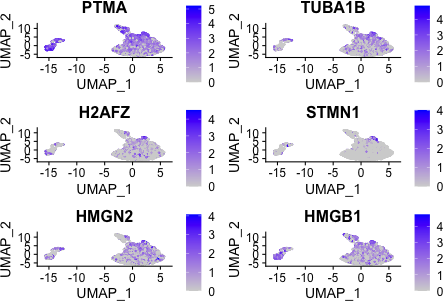
\includegraphics{figures/cluster-annotation-10-1.png}
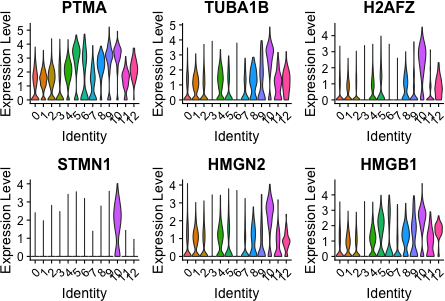
\includegraphics{figures/cluster-annotation-10-2.png}

\begin{longtable}[]{@{}lllrrrrrrrll@{}}
\toprule
\begin{minipage}[b]{0.09\columnwidth}\raggedright
\strut
\end{minipage} & \begin{minipage}[b]{0.09\columnwidth}\raggedright
ID\strut
\end{minipage} & \begin{minipage}[b]{0.09\columnwidth}\raggedright
Description\strut
\end{minipage} & \begin{minipage}[b]{0.01\columnwidth}\raggedleft
setSize\strut
\end{minipage} & \begin{minipage}[b]{0.02\columnwidth}\raggedleft
enrichmentScore\strut
\end{minipage} & \begin{minipage}[b]{0.01\columnwidth}\raggedleft
NES\strut
\end{minipage} & \begin{minipage}[b]{0.01\columnwidth}\raggedleft
pvalue\strut
\end{minipage} & \begin{minipage}[b]{0.01\columnwidth}\raggedleft
p.adjust\strut
\end{minipage} & \begin{minipage}[b]{0.01\columnwidth}\raggedleft
qvalues\strut
\end{minipage} & \begin{minipage}[b]{0.01\columnwidth}\raggedleft
rank\strut
\end{minipage} & \begin{minipage}[b]{0.05\columnwidth}\raggedright
leading\_edge\strut
\end{minipage} & \begin{minipage}[b]{0.30\columnwidth}\raggedright
core\_enrichment\strut
\end{minipage}\tabularnewline
\midrule
\endhead
\begin{minipage}[t]{0.09\columnwidth}\raggedright
Embryonic prefrontal cortex, Normal, Neural progenitor cell\strut
\end{minipage} & \begin{minipage}[t]{0.09\columnwidth}\raggedright
Embryonic prefrontal cortex, Normal, Neural progenitor cell\strut
\end{minipage} & \begin{minipage}[t]{0.09\columnwidth}\raggedright
Embryonic prefrontal cortex, Normal, Neural progenitor cell\strut
\end{minipage} & \begin{minipage}[t]{0.01\columnwidth}\raggedleft
49\strut
\end{minipage} & \begin{minipage}[t]{0.02\columnwidth}\raggedleft
0.648\strut
\end{minipage} & \begin{minipage}[t]{0.01\columnwidth}\raggedleft
3.23\strut
\end{minipage} & \begin{minipage}[t]{0.01\columnwidth}\raggedleft
0.000\strut
\end{minipage} & \begin{minipage}[t]{0.01\columnwidth}\raggedleft
0.000\strut
\end{minipage} & \begin{minipage}[t]{0.01\columnwidth}\raggedleft
0.000\strut
\end{minipage} & \begin{minipage}[t]{0.01\columnwidth}\raggedleft
73\strut
\end{minipage} & \begin{minipage}[t]{0.05\columnwidth}\raggedright
tags=69\%, list=24\%, signal=63\%\strut
\end{minipage} & \begin{minipage}[t]{0.30\columnwidth}\raggedright
H2AFZ/TUBA1B/CKS2/HMGN2/PTTG1/TOP2A/HIST1H4C/KPNA2/DUT/CCNB1/CDC20/BIRC5/TUBB4B/CCNB2/CDK1/ZWINT/CENPU/NUSAP1/RRM2/UBE2C/CENPW/PCNA/RPA3/CENPF/RRM1/MAD2L1/UBE2T/TMPO/DTYMK/HMGB2/RNASEH2A/CDKN3/DHFR/PBK\strut
\end{minipage}\tabularnewline
\begin{minipage}[t]{0.09\columnwidth}\raggedright
Large intestine, Normal, MKI67+ progenitor cell\strut
\end{minipage} & \begin{minipage}[t]{0.09\columnwidth}\raggedright
Large intestine, Normal, MKI67+ progenitor cell\strut
\end{minipage} & \begin{minipage}[t]{0.09\columnwidth}\raggedright
Large intestine, Normal, MKI67+ progenitor cell\strut
\end{minipage} & \begin{minipage}[t]{0.01\columnwidth}\raggedleft
20\strut
\end{minipage} & \begin{minipage}[t]{0.02\columnwidth}\raggedleft
0.708\strut
\end{minipage} & \begin{minipage}[t]{0.01\columnwidth}\raggedleft
2.80\strut
\end{minipage} & \begin{minipage}[t]{0.01\columnwidth}\raggedleft
0.000\strut
\end{minipage} & \begin{minipage}[t]{0.01\columnwidth}\raggedleft
0.000\strut
\end{minipage} & \begin{minipage}[t]{0.01\columnwidth}\raggedleft
0.000\strut
\end{minipage} & \begin{minipage}[t]{0.01\columnwidth}\raggedleft
51\strut
\end{minipage} & \begin{minipage}[t]{0.05\columnwidth}\raggedright
tags=75\%, list=17\%, signal=67\%\strut
\end{minipage} & \begin{minipage}[t]{0.30\columnwidth}\raggedright
PTTG1/TOP2A/HIST1H4C/TK1/CCNB1/CDC20/BIRC5/CCNB2/CDK1/NUSAP1/RRM2/UBE2C/CENPW/CENPF/UBE2T\strut
\end{minipage}\tabularnewline
\begin{minipage}[t]{0.09\columnwidth}\raggedright
Fetal gonad, Normal, Endothelial cell\strut
\end{minipage} & \begin{minipage}[t]{0.09\columnwidth}\raggedright
Fetal gonad, Normal, Endothelial cell\strut
\end{minipage} & \begin{minipage}[t]{0.09\columnwidth}\raggedright
Fetal gonad, Normal, Endothelial cell\strut
\end{minipage} & \begin{minipage}[t]{0.01\columnwidth}\raggedleft
24\strut
\end{minipage} & \begin{minipage}[t]{0.02\columnwidth}\raggedleft
0.558\strut
\end{minipage} & \begin{minipage}[t]{0.01\columnwidth}\raggedleft
2.34\strut
\end{minipage} & \begin{minipage}[t]{0.01\columnwidth}\raggedleft
0.000\strut
\end{minipage} & \begin{minipage}[t]{0.01\columnwidth}\raggedleft
0.000\strut
\end{minipage} & \begin{minipage}[t]{0.01\columnwidth}\raggedleft
0.000\strut
\end{minipage} & \begin{minipage}[t]{0.01\columnwidth}\raggedleft
58\strut
\end{minipage} & \begin{minipage}[t]{0.05\columnwidth}\raggedright
tags=54\%, list=19\%, signal=48\%\strut
\end{minipage} & \begin{minipage}[t]{0.30\columnwidth}\raggedright
STMN1/H2AFZ/TUBB/HMGN2/PTTG1/HMGB1/HIST1H4C/PTMA/BIRC5/CENPU/RANBP1/DTYMK/IDH2\strut
\end{minipage}\tabularnewline
\begin{minipage}[t]{0.09\columnwidth}\raggedright
Lung, Normal, FOXN4+ cell\strut
\end{minipage} & \begin{minipage}[t]{0.09\columnwidth}\raggedright
Lung, Normal, FOXN4+ cell\strut
\end{minipage} & \begin{minipage}[t]{0.09\columnwidth}\raggedright
Lung, Normal, FOXN4+ cell\strut
\end{minipage} & \begin{minipage}[t]{0.01\columnwidth}\raggedleft
16\strut
\end{minipage} & \begin{minipage}[t]{0.02\columnwidth}\raggedleft
0.496\strut
\end{minipage} & \begin{minipage}[t]{0.01\columnwidth}\raggedleft
1.80\strut
\end{minipage} & \begin{minipage}[t]{0.01\columnwidth}\raggedleft
0.011\strut
\end{minipage} & \begin{minipage}[t]{0.01\columnwidth}\raggedleft
0.041\strut
\end{minipage} & \begin{minipage}[t]{0.01\columnwidth}\raggedleft
0.029\strut
\end{minipage} & \begin{minipage}[t]{0.01\columnwidth}\raggedleft
123\strut
\end{minipage} & \begin{minipage}[t]{0.05\columnwidth}\raggedright
tags=81\%, list=40\%, signal=51\%\strut
\end{minipage} & \begin{minipage}[t]{0.30\columnwidth}\raggedright
TYMS/PTMA/CDK1/PTGES3/RANBP1/UBE2T/TMEM106C/DHFR/EIF2S2/SNRPG/OAT/ENO1/MAZ\strut
\end{minipage}\tabularnewline
\bottomrule
\end{longtable}

\hypertarget{other}{%
\subsubsection{Other}\label{other}}

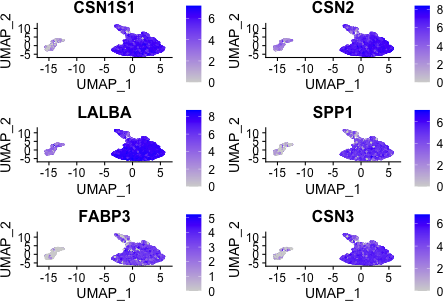
\includegraphics{figures/cluster-annotation-other-1.png}
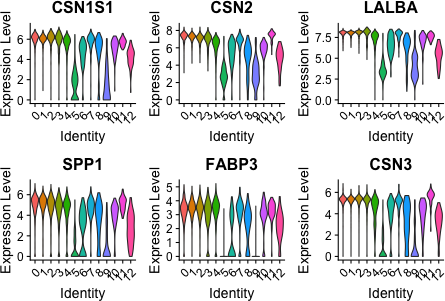
\includegraphics{figures/cluster-annotation-other-2.png}

\begin{longtable}[]{@{}llrrrrrr@{}}
\toprule
ID & Description & setSize & enrichmentScore & NES & pvalue & p.adjust &
qvalues\tabularnewline
\midrule
\endhead
\bottomrule
\end{longtable}

\hypertarget{summary-of-clusters}{%
\subsection{Summary of Clusters}\label{summary-of-clusters}}

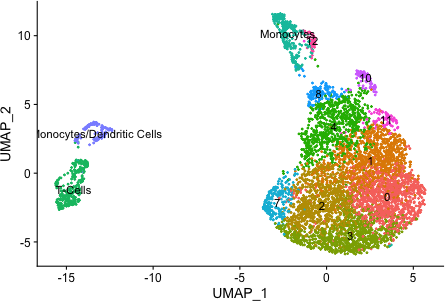
\includegraphics{figures/cluster-summary-1.png}

\begin{longtable}[]{@{}lr@{}}
\caption{Cell proportions in each cluster}\tabularnewline
\toprule
Var1 & Freq\tabularnewline
\midrule
\endfirsthead
\toprule
Var1 & Freq\tabularnewline
\midrule
\endhead
0 & 0.187\tabularnewline
1 & 0.165\tabularnewline
2 & 0.154\tabularnewline
3 & 0.150\tabularnewline
4 & 0.123\tabularnewline
T-Cells & 0.053\tabularnewline
Monocytes & 0.046\tabularnewline
7 & 0.036\tabularnewline
8 & 0.024\tabularnewline
Monocytes/Dendritic Cells & 0.024\tabularnewline
10 & 0.017\tabularnewline
11 & 0.014\tabularnewline
12 & 0.009\tabularnewline
\bottomrule
\end{longtable}

, \#\# Analysis of clusters

\begin{longtable}[]{@{}lrrrrrll@{}}
\caption{Clusters of genes of interest}\tabularnewline
\toprule
& p\_val & avg\_logFC & pct.1 & pct.2 & p\_val\_adj & cluster &
gene\tabularnewline
\midrule
\endfirsthead
\toprule
& p\_val & avg\_logFC & pct.1 & pct.2 & p\_val\_adj & cluster &
gene\tabularnewline
\midrule
\endhead
FASN & 0 & 0.660 & 0.855 & 0.755 & 0 & 7 & FASN\tabularnewline
FASN1 & 0 & 1.439 & 1.000 & 0.755 & 0 & 11 & FASN\tabularnewline
ACLY & 0 & 0.845 & 0.713 & 0.286 & 0 & 11 & ACLY\tabularnewline
CSN3 & 0 & 0.577 & 1.000 & 0.935 & 0 & 11 & CSN3\tabularnewline
\bottomrule
\end{longtable}

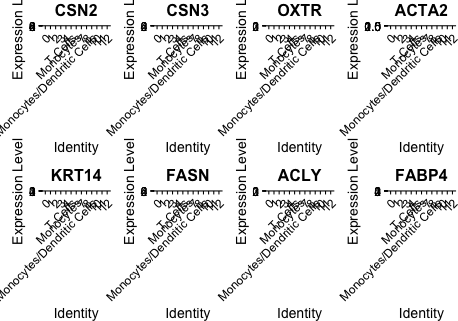
\includegraphics{figures/feature-analysis-1.png}
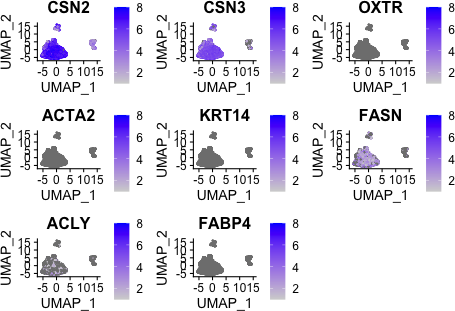
\includegraphics{figures/feature-analysis-2.png}
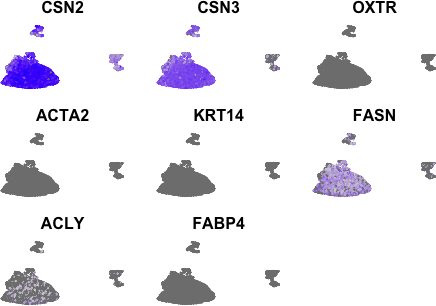
\includegraphics{figures/feature-analysis-3.png}
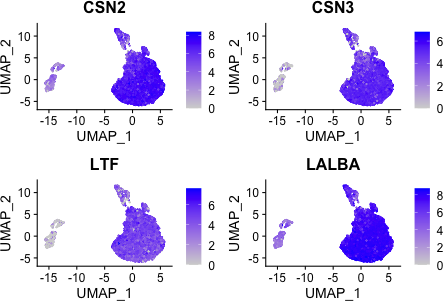
\includegraphics{figures/feature-analysis-4.png}
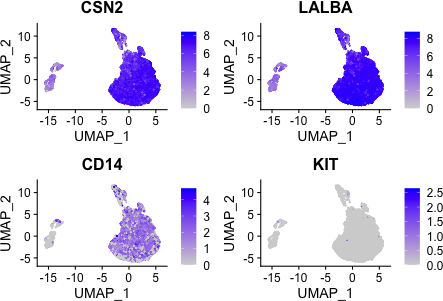
\includegraphics{figures/feature-analysis-5.png}
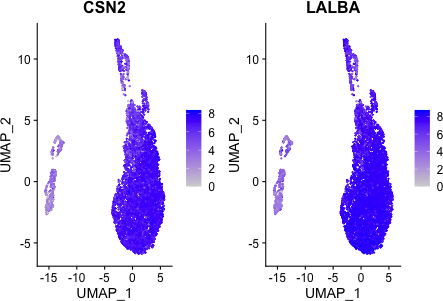
\includegraphics{figures/feature-analysis-6.png}
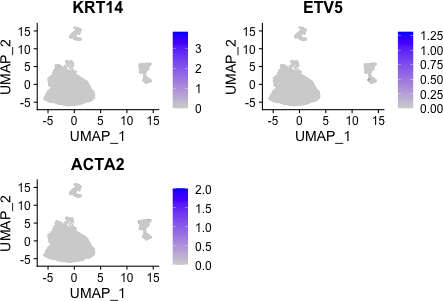
\includegraphics{figures/feature-analysis-7.png}
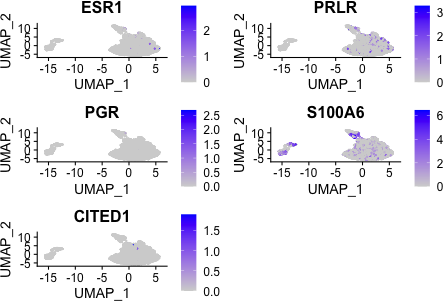
\includegraphics{figures/feature-analysis-8.png}
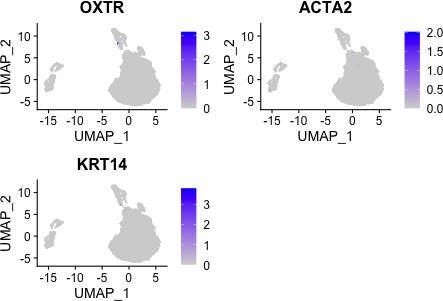
\includegraphics{figures/feature-analysis-9.png}
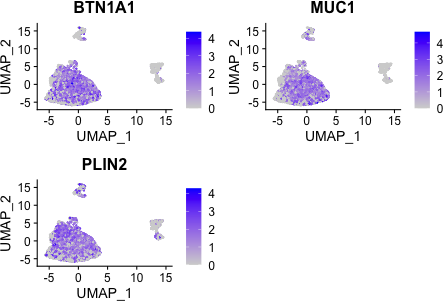
\includegraphics{figures/feature-analysis-10.png}
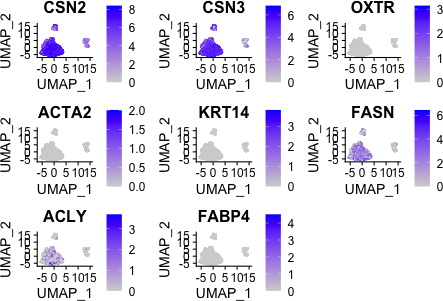
\includegraphics{figures/feature-analysis-11.png}
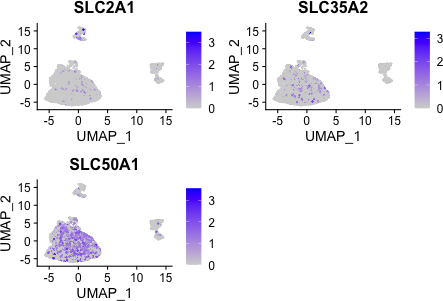
\includegraphics{figures/feature-analysis-12.png}
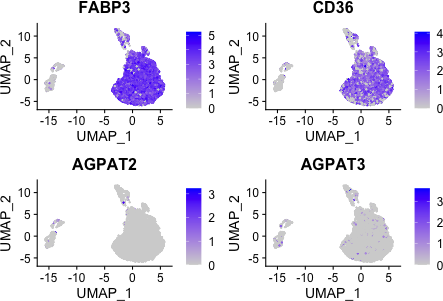
\includegraphics{figures/feature-analysis-13.png}
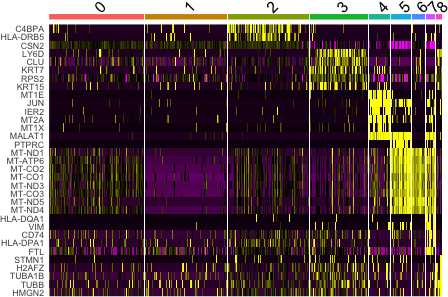
\includegraphics{figures/feature-analysis-14.png}
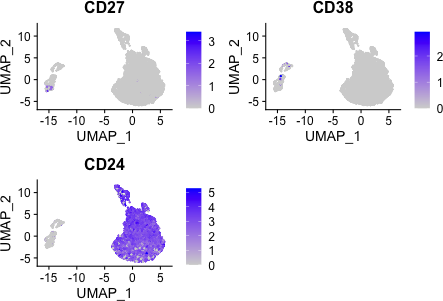
\includegraphics{figures/feature-analysis-15.png}
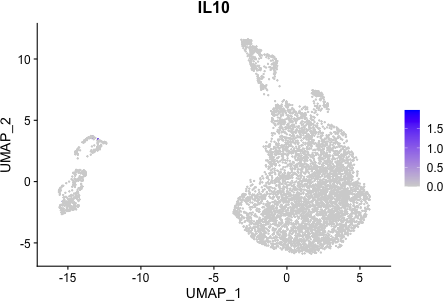
\includegraphics{figures/feature-analysis-16.png}
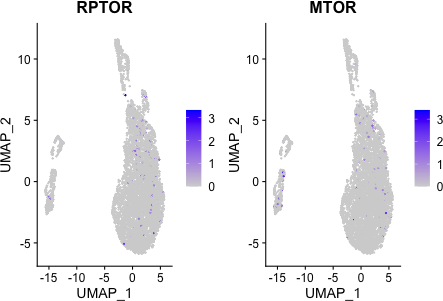
\includegraphics{figures/feature-analysis-17.png}
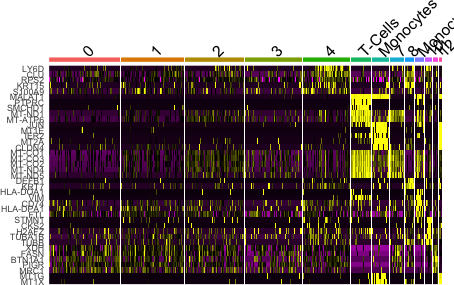
\includegraphics{figures/feature-analysis-18.png}

\hypertarget{session-information}{%
\section{Session Information}\label{session-information}}

\begin{Shaded}
\begin{Highlighting}[]
\KeywordTok{sessionInfo}\NormalTok{()}
\end{Highlighting}
\end{Shaded}

\begin{verbatim}
## R version 4.0.2 (2020-06-22)
## Platform: x86_64-apple-darwin17.0 (64-bit)
## Running under: macOS  10.16
## 
## Matrix products: default
## BLAS:   /Library/Frameworks/R.framework/Versions/4.0/Resources/lib/libRblas.dylib
## LAPACK: /Library/Frameworks/R.framework/Versions/4.0/Resources/lib/libRlapack.dylib
## 
## locale:
## [1] en_US.UTF-8/en_US.UTF-8/en_US.UTF-8/C/en_US.UTF-8/en_US.UTF-8
## 
## attached base packages:
## [1] stats     graphics  grDevices utils     datasets  methods   base     
## 
## other attached packages:
## [1] ggplot2_3.3.3          clusterProfiler_3.16.1 Seurat_3.2.3          
## [4] tibble_3.0.4           dplyr_1.0.2            tidyr_1.1.2           
## [7] knitr_1.30            
## 
## loaded via a namespace (and not attached):
##   [1] fastmatch_1.1-0       plyr_1.8.6            igraph_1.2.6         
##   [4] lazyeval_0.2.2        splines_4.0.2         BiocParallel_1.22.0  
##   [7] listenv_0.8.0         scattermore_0.7       urltools_1.7.3       
##  [10] digest_0.6.27         htmltools_0.5.0       GOSemSim_2.14.2      
##  [13] viridis_0.5.1         magick_2.5.2          GO.db_3.11.4         
##  [16] magrittr_2.0.1        memoise_1.1.0         tensor_1.5           
##  [19] cluster_2.1.0         ROCR_1.0-11           limma_3.44.3         
##  [22] globals_0.14.0        graphlayouts_0.7.1    matrixStats_0.57.0   
##  [25] vroom_1.3.2           prettyunits_1.1.1     enrichplot_1.8.1     
##  [28] colorspace_2.0-0      blob_1.2.1            ggrepel_0.9.0        
##  [31] xfun_0.19             crayon_1.3.4          jsonlite_1.7.2       
##  [34] scatterpie_0.1.5      spatstat_1.64-1       spatstat.data_1.7-0  
##  [37] survival_3.2-7        zoo_1.8-8             glue_1.4.2           
##  [40] polyclip_1.10-0       gtable_0.3.0          leiden_0.3.6         
##  [43] future.apply_1.6.0    BiocGenerics_0.34.0   abind_1.4-5          
##  [46] scales_1.1.1          DOSE_3.14.0           DBI_1.1.0            
##  [49] miniUI_0.1.1.1        Rcpp_1.0.5            progress_1.2.2       
##  [52] viridisLite_0.3.0     xtable_1.8-4          gridGraphics_0.5-1   
##  [55] reticulate_1.18       europepmc_0.4         bit_4.0.4            
##  [58] rsvd_1.0.3            stats4_4.0.2          htmlwidgets_1.5.3    
##  [61] httr_1.4.2            fgsea_1.14.0          RColorBrewer_1.1-2   
##  [64] ellipsis_0.3.1        ica_1.0-2             pkgconfig_2.0.3      
##  [67] farver_2.0.3          uwot_0.1.10           deldir_0.2-3         
##  [70] ggplotify_0.0.5       tidyselect_1.1.0      labeling_0.4.2       
##  [73] rlang_0.4.10          reshape2_1.4.4        later_1.1.0.1        
##  [76] AnnotationDbi_1.50.3  munsell_0.5.0         tools_4.0.2          
##  [79] downloader_0.4        generics_0.1.0        RSQLite_2.2.1        
##  [82] ggridges_0.5.2        evaluate_0.14         stringr_1.4.0        
##  [85] fastmap_1.0.1         yaml_2.2.1            goftest_1.2-2        
##  [88] bit64_4.0.5           fitdistrplus_1.1-3    tidygraph_1.2.0      
##  [91] purrr_0.3.4           RANN_2.6.1            ggraph_2.0.4         
##  [94] pbapply_1.4-3         future_1.21.0         nlme_3.1-151         
##  [97] mime_0.9              xml2_1.3.2            DO.db_2.9            
## [100] compiler_4.0.2        plotly_4.9.2.2        curl_4.3             
## [103] png_0.1-7             spatstat.utils_1.17-0 tweenr_1.0.1         
## [106] stringi_1.5.3         highr_0.8             RSpectra_0.16-0      
## [109] lattice_0.20-41       Matrix_1.3-0          vctrs_0.3.6          
## [112] pillar_1.4.7          lifecycle_0.2.0       BiocManager_1.30.10  
## [115] triebeard_0.3.0       lmtest_0.9-38         RcppAnnoy_0.0.18     
## [118] data.table_1.13.6     cowplot_1.1.1         irlba_2.3.3          
## [121] httpuv_1.5.4          patchwork_1.1.1       qvalue_2.20.0        
## [124] R6_2.5.0              promises_1.1.1        KernSmooth_2.23-18   
## [127] gridExtra_2.3         IRanges_2.22.2        parallelly_1.22.0    
## [130] codetools_0.2-18      MASS_7.3-53           withr_2.3.0          
## [133] sctransform_0.3.2     S4Vectors_0.26.1      hms_0.5.3            
## [136] mgcv_1.8-33           parallel_4.0.2        grid_4.0.2           
## [139] rpart_4.1-15          rvcheck_0.1.8         rmarkdown_2.6        
## [142] Rtsne_0.15            ggforce_0.3.2         Biobase_2.48.0       
## [145] shiny_1.5.0
\end{verbatim}

\hypertarget{refs}{}
\leavevmode\hypertarget{ref-Macosko2015}{}%
Macosko, Evan Z., Anindita Basu, Rahul Satija, James Nemesh, Karthik
Shekhar, Melissa Goldman, Itay Tirosh, et al. 2015. ``Highly parallel
genome-wide expression profiling of individual cells using nanoliter
droplets.'' \emph{Cell} 161 (5). Elsevier: 1202--14.
\url{https://doi.org/10.1016/j.cell.2015.05.002}.

\leavevmode\hypertarget{ref-MartinCarli2020}{}%
Martin Carli, Jayne F., G. Devon Trahan, Kenneth L. Jones, Nicole
Hirsch, Kristy P. Rolloff, Emily Z. Dunn, Jacob E. Friedman, et al.
2020. ``Single Cell RNA Sequencing of Human Milk-Derived Cells Reveals
Sub-Populations of Mammary Epithelial Cells with Molecular Signatures of
Progenitor and Mature States: a Novel, Non-invasive Framework for
Investigating Human Lactation Physiology.'' \emph{Journal of Mammary
Gland Biology and Neoplasia}. Journal of Mammary Gland Biology;
Neoplasia. \url{https://doi.org/10.1007/s10911-020-09466-z}.

\leavevmode\hypertarget{ref-Zhang2019a}{}%
Zhang, Xinxin, Yujia Lan, Jinyuan Xu, Fei Quan, Erjie Zhao, Chunyu Deng,
Tao Luo, et al. 2019. ``CellMarker: A manually curated resource of cell
markers in human and mouse.'' \emph{Nucleic Acids Research} 47 (D1).
Oxford University Press: D721--D728.
\url{https://doi.org/10.1093/nar/gky900}.

\end{document}
